\documentclass[11pt,a4paper]{article}
\usepackage[T1]{fontenc}
\usepackage[utf8]{inputenc}
\usepackage{lmodern,microtype}
\usepackage[margin=25mm,headheight=15pt]{geometry}
\usepackage{amsmath,amssymb,amsthm,mathtools}
\usepackage{booktabs,longtable,tabularx,array,ragged2e}
\usepackage{xcolor,listings,enumitem,fancyhdr,titlesec}
\usepackage{needspace}
\usepackage{tocloft}
\setlength{\cftbeforesecskip}{2.5pt}
\usepackage{tikz}
\usetikzlibrary{arrows.meta,positioning,calc}
\usepackage[most]{tcolorbox}
\usepackage{xurl}
\usepackage[colorlinks=true,linkcolor=ink,citecolor=ink,urlcolor=ink]{hyperref}
\definecolor{ink}{HTML}{183B56}
\definecolor{accent}{HTML}{247F86}
\definecolor{pale}{HTML}{F0F5F7}
\definecolor{muted}{HTML}{52606B}
\hypersetup{pdftitle={Concord: A Mathematical Language with Certified Computation},pdfauthor={ChatGPT},pdfsubject={Second-iteration proof-language proposal for the Brainstorm campaign}}
\setlength{\parindent}{0pt}
\setlength{\parskip}{.48em}
\setlength{\emergencystretch}{2em}
\setcounter{tocdepth}{1}
\hypersetup{bookmarksdepth=2}
\setlist{nosep,leftmargin=1.7em}
\renewcommand{\arraystretch}{1.18}
\newcolumntype{L}[1]{>{\RaggedRight\arraybackslash}p{#1}}
\newcolumntype{Y}{>{\RaggedRight\arraybackslash}X}
\titleformat{\section}{\Large\bfseries\color{ink}}{\thesection}{.65em}{}
\titleformat{\subsection}{\large\bfseries\color{ink}}{\thesubsection}{.65em}{}
\titleformat{\subsubsection}{\normalsize\bfseries}{\thesubsubsection}{.65em}{}
\titlespacing*{\section}{0pt}{2.0ex plus 1ex}{.8ex}
\titlespacing*{\subsection}{0pt}{1.6ex plus .5ex}{.45ex}
\pagestyle{fancy}
\fancyhf{}
\fancyhead[L]{\small\color{muted}Concord \;|\; Mathematical reasoning and certified computation}
\fancyfoot[L]{\small\color{muted}Second brainstorm iteration \;\textbullet\; September 2026}
\fancyfoot[R]{\small\thepage}
\renewcommand{\headrulewidth}{.3pt}
\lstset{basicstyle=\ttfamily\small,columns=fullflexible,keepspaces=true,
 breaklines=true,breakatwhitespace=false,showstringspaces=false,
 backgroundcolor=\color{pale},frame=single,rulecolor=\color{pale},
 xleftmargin=.5em,xrightmargin=.5em,framesep=5pt,
 aboveskip=.7em,belowskip=.7em,tabsize=2}
\newcommand{\code}[1]{\texttt{\detokenize{#1}}}
\newcommand{\R}{\mathbb R}
\newcommand{\C}{\mathbb C}
\newcommand{\Q}{\mathbb Q}
\newcommand{\Z}{\mathbb Z}
\newcommand{\N}{\mathbb N}
\newcommand{\sem}[1]{\llbracket #1\rrbracket}
\newcommand{\Spec}{\mathsf{Spec}}
\newcommand{\Dom}{\mathsf{Dom}}
\newcommand{\EqOn}{\mathsf{EqOn}}
\newcommand{\J}{\mathsf{J}}
\newcommand{\bref}[2]{\href{#1}{#2}}
\newtcolorbox{decisionbox}[1][]{colback=pale,colframe=accent,boxrule=.5pt,
 arc=1pt,left=9pt,right=9pt,top=6pt,bottom=6pt,breakable,#1}
\newtheorem{proposition}{Proposition}[section]
\newtheorem{theorem}[proposition]{Theorem}
\newtheorem{definition}[proposition]{Definition}
\newtheorem{example}[proposition]{Example}
\theoremstyle{remark}
\newtheorem{remark}[proposition]{Remark}

\begin{document}
\begin{titlepage}
\vspace*{10mm}
{\small\sffamily\bfseries\color{accent}BRAINSTORM CAMPAIGN \quad / \quad SECOND ITERATION\par}
\vspace{13mm}
{\fontsize{35}{40}\selectfont\bfseries\color{ink}Concord\par}
\vspace{4mm}
{\LARGE\bfseries A Mathematical Language\\with Certified Computation\par}
\vspace{9mm}
{\large From readable proof steps to a domain-aware,\\proof-producing computer algebra workspace\par}
\vspace{11mm}
\begin{decisionbox}
\textbf{Central proposal.} Write the mathematical choices; let verified algorithms
construct their consequences; retain the exact domains and specifications of every
computed object. A calculation is not merely an expression returned by a solver:
it is an object accompanied by a precisely stated theorem about that object.
\end{decisionbox}
\vspace{8mm}
\textbf{Prepared for} Vladimir Reshetnikov's Brainstorm campaign\\
\textbf{Prepared by} ChatGPT\\
\textbf{Date} September 5, 2026, Pacific time
\vfill
\small
\textbf{Status.} This is a research and engineering design, not an implemented
language. It is based on a close reading of both requested synthesis reports,
static inspection of selected committed ProveIt and Leant sources, and primary
literature on verified computation. The mathematical examples include explicit
proofs. The accompanying Python checks were executed; they are not Lean proofs.
No new Lean compiler, CAS integration, or human-subject evaluation is claimed.
\end{titlepage}

\begin{abstract}
The first Brainstorm iteration reached a useful consensus: retain Lean's checking
foundation, make mathematical steps visible, elaborate omissions into scoped
obligations, preserve the intended statement, and retain evidence rather than
repeat open-ended discovery. A second iteration should not merely rename this
architecture. This article proposes a specific extension: a mathematical language
whose central objects include \emph{certified computations}, not only proof goals.
The resulting system, provisionally called Concord, combines a structured proof
surface with a computer algebra workspace built around formally specified
algorithms, executable representations, and kernel-checkable evidence.

Its distinctive features are contracts that distinguish an identity from a
complete solution, domain-preserving simplification, explicit branch coverage,
composable representation packages, and a shared interface for verified
algorithms, certificate-producing external CAS tools, Lean tactics, and Leant's
term synthesis. The main worked example derives the polynomial recurrence for
all derivatives of both real Lambert branches, separating a reusable symbolic
calculation from local analytic hypotheses. Further examples cover rational
cancellation, complete root solving, finite binomial transforms in additive
commutative groups, radical denesting, and finite jets of formal series.

The proposal resolves concrete questions raised by the two syntheses, specifies
trust and replay boundaries, gives a bounded implementation plan, and supplies
negative tests that distinguish mathematical validity from plausible computation.
Its central empirical hypothesis is that attaching precise, reusable meaning to
computations reduces both authoring friction and maintenance cost more effectively
than hiding additional tactic lines. That hypothesis remains to be tested against
ordinary Lean supplied with exactly the same libraries and algorithms.
\end{abstract}
\begingroup
\small
\setlength{\parskip}{0pt}
\tableofcontents
\endgroup
\clearpage

\Needspace{7\baselineskip}
\section{The proposal in one argument}
\label{sec:thesis}
A mathematician often writes a proof in a mixture of logical and computational
moves: choose a substitution, rewrite a sum, differentiate an identity, solve a
polynomial equation, inspect a few coefficients, conjecture a recurrence, and
then prove that recurrence for every index. A proof assistant can represent all
these activities, but the user interface need not force them all into the same
shape of ``a goal followed by tactics.'' Conversely, a computer algebra system
can manipulate expressions without making the precise scope of each answer
conveniently available to subsequent reasoning.

I propose a workspace in which a \emph{mathematical claim} and a \emph{computed
mathematical object with a specification} are equally natural units. The language
should support both
\[
 \text{establish }P
 \qquad\text{and}\qquad
 \text{construct }y\text{ satisfying }\Spec(x,y).
\]
The first asks for evidence of a fixed proposition. The second asks for data and
for evidence of a property of that exact data. The second operation is not safely
replaced by finding an inhabitant of the output type.

For example, a returned list of roots may contain only genuine roots while
omitting half the solution set. A factorization may multiply back to the input
without being irreducible. An antiderivative may be correct on one component of
a domain without specifying every antiderivative on the whole domain. A
truncated series may satisfy an equation modulo a power of its variable without
solving the equation as an infinite series. These are not peripheral exceptions.
They determine what subsequent mathematics may legitimately conclude.

\begin{decisionbox}
\textbf{Design commitment.} Every computational verb has an exact result contract.
The language never upgrades ``a verified candidate'' to ``the complete answer''
unless the stronger property has its own evidence. Domains, branches, coefficient
structures, and approximation relations belong to the contract, not to a warning
printed after the answer.
\end{decisionbox}

The proposal retains the first-round architecture rather than replacing it.
Concord is initially a Lean-hosted mathematical interface, with an ordinary Lean
frontend and a structured document frontend over shared methods. Its foundation
is not a new logic. Its new work lies in the organization of computations and
their specifications, in predictable transport between representations, and in
the authoring experience around those operations.

This also changes what should be automated. A system should be particularly good
at taking a \emph{chosen} substitution, recurrence ansatz, or representation and
producing all the consequences that follow mechanically. It may suggest a better
choice, but adopting that suggestion is a visible change to the mathematical
plan. A proof which is shorter because the system silently chose a different
problem is not a success.

\Needspace{4\baselineskip}
\subsection{What ``human-scale'' should mean}
The objective is not to mimic every sentence of informal prose. It is to let the
reader see the invariant, the useful representation, the decisive reduction, and
the reason the calculation applies. The details may then be expanded where they
matter. A domain condition such as $w\ne-1$ is visually prominent in a Lambert
calculation because it controls the pole; the proof that a positive exponential
is nonzero can normally remain collapsed.

Exploration and exposition should differ. During exploration, the workspace can
hold several candidate normal forms and competing proof plans. In the published
argument, it retains the accepted object, its specification, and a concise reason
for its use. The discarded candidates may remain in an optional private search
log. They are not automatically part of the proof document.

Nor should the system insist on prose when a formula or a short Lean expression
is already better. Existing theorem applications and calculation blocks remain
first-class input. A new surface earns its place by improving the expression or
understanding of a mathematical decision, not by translating every line into
English.

\Needspace{7\baselineskip}
\section{What the two syntheses establish---and what they leave open}
\label{sec:reading}
\Needspace{4\baselineskip}
\subsection{A close-reading position}
The two requested reports are complementary. \emph{Mathematical Ideas, Checked
Evidence}, here called synthesis A, develops a six-commitment common architecture,
careful acceptance distinctions, a substantial static review of Leant, and
specific next-round experiments. \emph{Nine Blueprints for a Mathematician's Proof
Language over Lean}, synthesis B, supplies a finer feature matrix, a lexical
corpus audit, the annotated-theorem proposal, and a strong challenge to the idea
that new syntax is the main missing ingredient~\cite{synA,synB}.

The most important shared conclusions should be treated as the starting point,
not as this article's innovations: a fixed resolved statement; ordered dependent
contexts; explicit mathematical choices; reusable theorem-backed methods;
independent checking of candidates; evidence attached to all asserted claims;
and fair comparison with refactored Lean. The individual proposals are discussed
here through the syntheses' detailed crosswalks, rather than presented as nine
newly replicated implementation studies~\cite{synA,synB}.

There are also places where a second-round design should be more precise than
an attractive slogan. A statement seal is not necessarily obtained by one
isolated elaboration pass: types, instances, and universe constraints can remain
interdependent. The meaningful requirement is a checked, immutable semantic
boundary before an external proof producer receives authority to solve the
request. An abstraction-safety flag is useful evidence \emph{about a search
procedure}, but is not itself a kernel proof of a negative mathematical claim.
A measured frequency of cast-like lines is not a measurement of removable work.
These distinctions govern the design below.

\Needspace{4\baselineskip}
\subsection{How this proposal differs from another first-round blueprint}
\begin{longtable}{@{}L{.28\textwidth}L{.64\textwidth}@{}}
\toprule
Starting point in the syntheses & Additional decision in Concord \\
\midrule
\endhead
Typed assertions and an obligation ledger & Computed objects also carry contracts:
identity, domain equivalence, completeness, canonicality, or a specified error
relation. These contracts are not collapsed into a single status.\\
Certified representation views & A compositional interface fixes direction,
guards, semantic observations, and whether a route preserves or reflects a
property. Competing meaning-bearing routes require an explicit choice.\\
Definition authoring as an open problem & Start with definition packages for
partial expressions and executable polynomial representations, not a general
natural-language definition parser.\\
Methods as annotated theorems & Use ordinary theorems for logical assembly;
use verified algorithms or verified certificate checkers for computational
families. Give both the same result-contract interface.\\
Leant behind a typed boundary & Separate candidate generation, exact displayed-edit
replay, mathematical specification proof, and whole-document completion.\\
Retained evidence & Archive the exact target, accepted data, certificate inputs,
checker theorem, proof evidence, and environment. A computed answer is part of
the mathematical artifact, not just a tactic trace.\\
Shared-method evaluation & Add an algorithm-versus-interface ablation: a better CAS
backend and a better language must not receive credit for the same gain.\\
\bottomrule
\end{longtable}

\Needspace{4\baselineskip}
\subsection{What the repository examples actually show}
Three directly inspected ProveIt modules are especially informative.
\code{BinomialInversion.lean} separates integer-kernel algebra from transforms
on an arbitrary additive commutative group. Its final results already reuse a
triangular-kernel framework. \code{AutonomousIteratedDeriv.lean} isolates a local
chain-rule theorem whose differentiability assumptions apply only at values
actually reached by the solution. \code{LambertWHigherDerivatives.lean} combines
that theorem with explicit exponential, polynomial, and quotient-rule
calculations~\cite{pbinomial,pautonomous,plambert}.

The third module supplies the central new test in this article. The symbolic
calculation and the local analysis are already mathematically separated, but
there is an opportunity to give the former a reusable executable interface.
The new language should not hide or weaken the latter. This is a stronger test
than making an already available final theorem easier to invoke.

Synthesis B's audit classifies roughly one third of its tactic-like source
entries into families proposed for reconstruction, and synthesis A explicitly
warns against interpreting that figure as a savings estimate. I adopt that
warning. This article does not rerun the audit, claim that the sampled corpus was
compiled, or infer a percentage reduction in development time from source
frequencies~\cite{synA,synB}.

\Needspace{4\baselineskip}
\subsection{Source identity and scope of this review}
Both syntheses were read at Brainstorm revision \code{494be9d5}. The public refs
resolved during this review were ProveIt \code{24ce8bd7} and Leant
\code{3a40904b}. The syntheses also discuss a different local ProveIt snapshot
and uncommitted Leant work. Those observations remain attributed to the reports;
they are not silently recast as observations of the committed files inspected
here. Full revision identities and file locators appear in
Appendix~\ref{app:sources}.

\Needspace{7\baselineskip}
\section{A mathematical workspace, not a larger tactic vocabulary}
\label{sec:workspace}
\Needspace{4\baselineskip}
\subsection{The four kinds of persistent node}
The proposed intermediate representation has four principal kinds of mathematical
node. A \emph{claim} has a fixed proposition and evidence. An \emph{object} has a
fixed type, a chosen value, and its declared specification. A \emph{computation}
links input objects to output objects through a checked relation. A
\emph{scope} binds parameters, assumptions, definitions, notation, and local
representation policies. An operation may create several nodes at once.

The dependency structure is more than a graph of propositions. For example,
choosing a polynomial order affects a computed normal form; choosing a root
affects later functions; choosing a domain changes which substitutions are
legal. Those are data dependencies. They must be recorded even when two choices
happen to make the same proposition provable.

This gives a single workspace two useful directions. A backward request such as
``show this expression is nonnegative'' asks for a certificate meeting a fixed
goal. A forward request such as ``factor this polynomial over $\Q$'' produces a
candidate factor object and a theorem about it. A later proof can use that
object without rediscovering it or reparsing its printed form.

\Needspace{4\baselineskip}
\subsection{An inspectable semantic header}
Each declaration has a resolved header recording its binders, dependency order,
constants, instances, and chosen interpretations. The reader-facing view should
show the few choices that distinguish nearby mathematical statements: natural
versus integer subtraction, total versus partial division, formal versus analytic
series, and pointwise versus neighborhood equality.

This is not an algorithm for recovering the author's intention. A deterministic
rendering can disclose what was formalized; the author must still recognize
whether it is the desired statement. The renderer and source map need their own
tests. A hash of an elaborated expression identifies a record but does not make
the record intelligible.

Local conventions are lexical and explicit. For example, an author can declare
that an expression block uses partial real functions while the surrounding Lean
file continues to use its ordinary total operations. The system then inserts
proved interface lemmas at the boundary. It must not change the meaning of
existing Lean notation globally.

\Needspace{4\baselineskip}
\subsection{A small proposed surface}
The following is \emph{proposed syntax}, not executable Lean or an implemented
Concord parser:
\par\smallskip\noindent\begin{minipage}{\linewidth}
\begin{lstlisting}
context rational_functions:
  variable x : Real
  let f := partial (x^2 - 1) / (x - 1)

  calculate g := simplify f
    preserving domain
    by rational_normal_form

  have roots : solutions(f = 0) = {-1}
    by solve_completely over Real

  explain "Cancellation preserves the original missing point."
\end{lstlisting}
\end{minipage}\par\smallskip
The first command creates a mathematical object with a specified domain. The
calculation binds a new representation of the same partial function. The claim
about solutions requires a complete solution-set contract. The final line is
ordinary commentary, visibly distinguished from a formally asserted claim.

For a logical argument the surface stays close to a familiar structured proof:
\par\smallskip\noindent\begin{minipage}{\linewidth}
\begin{lstlisting}
proof:
  fix n
  induct n maintaining the identity on U
  case zero:
    conclude by the defining equation
  case successor n:
    fix x in U
    differentiate the induction identity near x
    conclude by the chain rule and the recurrence
\end{lstlisting}
\end{minipage}\par\smallskip
The maintained identity, the open set $U$, and the recurrence are bound typed
objects, not strings that a model resolves by plausibility. The short English
aliases are a presentation layer over stable references.

A narrow first grammar needs declarations, named claims, object bindings,
calculations, scopes, case splits, induction with a stated motive, and a Lean
escape block. It does not need unrestricted English theorem statements. The
extension beyond the syntheses is primarily the semantics of \code{calculate}
and of its output, not a proliferation of keywords.

\Needspace{4\baselineskip}
\subsection{Author-selected inputs versus reconstructible requirements}
The logical contract of a method remains an ordinary theorem where possible.
Its binders receive roles such as \emph{input}, \emph{choice}, and
\emph{requirement}. The distinction is contextual. A bijection can be routine in
one reindexing and the central idea in another. A ``requirement'' is never an
assertion that its proof is easy.

For long-term stability, I would register roles on a small project-owned wrapper
with a documented semantic interface. That wrapper may delegate to a changing
Mathlib theorem. This creates a modest, explicit maintenance cost, but avoids
making every upstream binder rename a language-API change. The wrapper's checked
type is authoritative; operational metadata is separately versioned. Positional
binder lists and automatic classification of every proposition as a side
condition are both too fragile.

Named methods constrain the accepted construction when their wording asserts a
method: ``by reindexing'' must actually supply a reindexing contract. An explicitly
open justification, such as ``by search,'' permits another proof of the same
claim. An alternative argument is welcome, but accepting it changes the displayed
reason rather than leaving an inaccurate explanation in place.

\Needspace{4\baselineskip}
\subsection{How the interface supports mathematical thought}
Suppose an author guesses a form $e^{-nw}P(w)/(1+w)^k$. The workspace can immediately
show its derivative, the denominator conditions, and the polynomial factor
needed to close the induction. The author sees whether the ansatz is stable under
the differential operator. This is a much more useful interaction than receiving
only a sequence of suggested quotient-rule tactics.

Similarly, a sum can be displayed as a function of its index region, with a chosen
map and its image. A failed reindexing can show the missing endpoint. A formal
series calculation can display exactly which coefficients have been determined.
The proof state remains available, but it is no longer the only representation
of progress.

Analogy is treated as checked reuse. ``Similarly for the lower branch'' instantiates
a known template with different branch hypotheses; the newly required inequality
is visible. Induction is treated as a mathematical invariant rather than an
instruction to manipulate whatever goal happened to be active. These mechanisms
do not certify a human mental process. They preserve a useful mathematical
explanation of the accepted argument.

\Needspace{7\baselineskip}
\section{Computation contracts: say exactly what was obtained}
\label{sec:contracts}
\Needspace{4\baselineskip}
\subsection{A result is a value together with a proposition about it}
For input $x:I$, output type $O(x)$, and a specification
$\Spec(x,y)$, the ideal mathematical result has the dependent type
\[
 \mathsf{Result}(x)=\{y:O(x)\mid\Spec(x,y)\}.
\]
An implementation may store a certificate from which the proof is reconstructed
rather than a directly serialized dependent pair. Nevertheless, the acceptance
boundary must establish the displayed specification for the \emph{exact} accepted
output. Verifying a similar expression, an earlier candidate, or the output of
a different renderer does not establish it.

There is no single universal specification for ``simplify,'' ``solve,'' or
``factor.'' The interface needs a small family of explicit contracts. A result
can carry several compatible properties, each with its own evidence. The
properties form a partial order under proved implications, not a universal ladder
on which every task receives one numerical confidence score.

\begin{longtable}{@{}L{.20\textwidth}L{.36\textwidth}L{.36\textwidth}@{}}
\toprule
Request & Minimal useful certificate & Additional property not implied \\
\midrule
\endhead
Rewrite an expression & Equality under a stated domain and interpretation &
Equality of domains; preferred form; minimal expression size.\\
Factor a polynomial & Product of returned factors equals the input &
Irreducibility, uniqueness conventions, or completeness over another field.\\
Find solutions & Every returned object satisfies the equation &
Every solution is returned; multiplicity; a canonical ordering.\\
Solve completely & Membership in the returned set is equivalent to the original
predicate & Efficient membership, finite enumeration, or preferred parametrization.\\
Compute a derivative & A derivative assertion on the stated domain &
Maximal differentiability domain or validity at excluded boundary points.\\
Integrate symbolically & The returned function has the requested derivative on a
domain & A definite integral formula or all antiderivatives on disconnected domains.\\
Compute a series jet & Equality of coefficients below a fixed order &
An infinite identity, convergence, or an analytic remainder estimate.\\
Enclose a value & Exact lower and upper bounds & Exact equality to a decimal or
minimal interval width.\\
Prove ideal membership & An exact identity $p=\sum_i h_i f_i$ in the specified
coefficient ring & A Gr\"obner basis, non-membership, or ideal membership over a
smaller coefficient ring.\\
Select a root & Its defining equation and selected branch condition &
Uniqueness without an additional theorem; executable selection from existence alone.\\
\bottomrule
\end{longtable}

These distinctions are mathematical rather than cosmetic. Davenport's study of
verified polynomial factorization explicitly separates checking a product identity
from verifying irreducibility~\cite{davenport}. Concord should make that
separation unavoidable in the result type, not merely repeat it in documentation.

\Needspace{4\baselineskip}
\subsection{Complete solutions are predicates before they are lists}
Let $P:A\to\mathsf{Prop}$ be the original solution predicate. A returned list $L$
can be certified by
\[
 \forall y,\;y\in L\Longrightarrow P(y).
\]
A complete finite answer needs the stronger property
\[
 \forall y,\;y\in L\Longleftrightarrow P(y).
\]
A system solving $a x=0$ over $\R$ cannot always return a finite list: when $a=0$
every real number is a solution. The result type should therefore permit a
symbolic set or a parameterized family, with a theorem characterizing its
membership. Enumeration is an additional representation choice.

For the parameterized example, a complete answer is
\[
 \{x\in\R:ax=0\}=
 \begin{cases}
   \R,&a=0,\\
   \{0\},&a\ne0.
 \end{cases}
\]
In the second case division by $a$ proves necessity, and substitution proves
sufficiency. In the first case multiplication by zero proves every $x$ is a
solution. The cases cover all $a$. A generic answer ``$x=0$'' with the unproved
condition $a\ne0$ is useful, but it is a \emph{conditional answer}, not the
complete parameterized solution.

Multiplicity is a separate contract. A set of polynomial zeros intentionally
forgets multiplicity; a multiset factorization does not. Over $\R$ and over $\C$
the zero sets may also differ. The solver does not infer a field merely because
one field produces a simpler answer.

\Needspace{4\baselineskip}
\subsection{Canonicality must be defined, not suggested by typography}
An algorithm can return any correct factor order unless an order is required.
An algebraic number can have many defining polynomials and isolating intervals.
A normal form is canonical only relative to specified conventions: coefficient
normalization, variable order, term order, algebraic extension, and an equality
notion. The interface should never display ``canonical'' simply because the
output is deterministic in one run.

For most proof steps, canonicality is unnecessary. A proof needs a convenient
representative with a transport theorem. Demanding a global canonical form can
increase checking cost and make the interface less stable. Concord therefore
asks for the weakest sufficient mathematical result, while retaining the
opportunity to request stronger properties explicitly.

\Needspace{4\baselineskip}
\subsection{Finite observations versus universal behavior}
A synthesized function may satisfy a test at a few inputs while failing its
intended universal law. Leant's separation between term construction and
behavioral assessment is directly relevant here. Its committed verification
wrapper explicitly records callback acceptance rather than a kernel or behavioral
certificate~\cite{lverify}. The syntheses also describe an uncommitted
candidate-bound proposition check; that observation is attributed to those
snapshots, not asserted as an API executed in this review~\cite{synA,synB}.

Concord records the proposition actually established. A proof of a finite test
conjunction certifies that conjunction. A proof of a universal law certifies the
law. Some universally quantified propositions over finite types are decidable;
the distinction is not the presence of a quantifier but the exact specification
and the evidence returned. A provisional data object can be explored under a
weaker tested property, but a published theorem cannot quietly consume the
unproved stronger one.

\Needspace{7\baselineskip}
\section{What a formally verified CAS would actually require}
\label{sec:cas}
\Needspace{4\baselineskip}
\subsection{Three implementation lanes, one logical interface}
The hybrid system should support three lanes while labeling their guarantees
honestly.

\textbf{Verified algorithm lane.} A function $a:I\to O$ is defined in the host
logic, and a theorem proves
\[
 \forall x,\;\Spec(x,a(x)).
\]
This is the appropriate target for stable computational building blocks:
polynomial arithmetic, a syntax-directed derivative algorithm on a specified
expression grammar, exact rational arithmetic, and truncated series operations.
Termination is established for the host definition or separately for the stated
algorithmic interface.

\textbf{Certified external-result lane.} An untrusted program returns $(y,c)$.
A host-defined checker $\mathsf{check}$ and its soundness theorem establish
\[
 \mathsf{check}(x,y,c)=\mathsf{true}\Longrightarrow\Spec(x,y).
\]
The search or factorization algorithm need not be verified. The accepted result
is nevertheless rigorous when the checker theorem and its actual application
are checked. This is a verified \emph{checking boundary}, not a claim that the
external CAS algorithm has been formally verified.

\textbf{Proof-producing symbolic lane.} A tactic or compiler constructs a proof
of $\Spec(x,y)$ directly using registered lemmas. A derivative expression can be
built recursively together with derivative evidence. Algebraic cleanup can then
use an existing proof-producing normalizer. Such a producer may remain logically
untrusted because the resulting term is checked at the exact requested type.
Its operational execution still requires appropriate isolation.

All three lanes can inhabit the same result contract. They differ in what is
proved about the program and in how a concrete execution acquires authority.
A practical system should use verified algorithms for its reusable core and
allow certificate-producing external services for expensive search. It should
not delay all useful interaction until an entire general-purpose CAS has been
reimplemented and verified.

\Needspace{4\baselineskip}
\subsection{The execution gap in ``the algorithm was proved correct''}
Suppose a verified function $a$ is compiled and an executable prints the value
$y$. The theorem $\Spec(x,a(x))$ alone does not prove $\Spec(x,y)$. One also needs
an accepted connection between the concrete returned data and $a(x)$.
There are several valid routes: kernel reduction identifies the values; a
proof-producing evaluator constructs the equality $a(x)=y$; or an independent
checker establishes the required specification directly from $x,y,c$.

This small distinction is central to a genuinely rigorous hybrid. Proof
annotations erased by a compiler do not make arbitrary executable output
self-authenticating. A formally verified source algorithm and a trusted native
execution mode are different guarantees. A deployment may intentionally trust
its compiler, but it must not describe that choice as the same trust boundary
as kernel-only checking.

Lean's current documentation makes the distinction observable: native computation
can introduce additional axiom dependencies, and current \code{native_decide}
uses a per-invocation axiom. A blacklist of one historical axiom name is therefore
not an adequate publication policy~\cite{leanaxioms}. The strict Concord profile
requires an explicit transitive allowlist. A separate performance-oriented profile
may permit additional computation assumptions, but the exported artifact and
reader view must state that choice.

Current Lean documentation also describes \code{cbv} as a proof-layer,
call-by-value-style simplification mechanism. This provides a relevant candidate
for evaluation of some verified computations without equating native execution
with proof. Availability and performance must be tested at the pinned project
toolchain; the moving manual is not a compatibility guarantee~\cite{leancbv}.

\Needspace{4\baselineskip}
\subsection{Reification is part of the proof boundary}
Efficient computation usually uses a representation different from the library's
semantic expression. Let $\mathsf{Rep}$ be a computable polynomial representation
and $\mathsf{denote}:\mathsf{Rep}\to\mathsf{Polynomial}(R)$ its interpretation.
A certificate about the representation becomes useful only after the bridge to
the original input has been established:
\[
 \mathsf{denote}(r)=p,\qquad
 \mathsf{check}(r,s,c)=\mathsf{true},\qquad
 \mathsf{check\_sound}:\cdots\Longrightarrow
   \Spec(\mathsf{denote}(r),\mathsf{denote}(s)).
\]
The importer must not trust that a printed variable name, coefficient string,
or CAS symbol happens to denote the intended Lean object. Variables need typed
identities; rational coefficients need exact numerators and denominators;
noncommutative expressions cannot be flattened into commutative polynomials.
A reification error is harmless only if the bridge to the fixed input is also
checked and the final result is checked against the original specification.

Useful sharing does not require an enormous universal symbolic-expression type.
Small domain-specific representations are preferable. A polynomial syntax can
have a complete, simple semantics. A derivative syntax can include a limited set
of differentiable operations and treat other functions as opaque atoms with
explicit derivative hypotheses. Failure to recognize an atom produces a located
unsupported result, not an invented identity.

\Needspace{4\baselineskip}
\subsection{What existing work can be reused}
There is substantial prior art for the computational half. Isabelle's Archive of
Formal Proofs contains verified univariate polynomial factorization, including
the Berlekamp--Zassenhaus development and associated square-free and rational
interfaces~\cite{berlekamp}. Rocq's Interval package supplies automated real
inequality and enclosure reasoning, including supported integral
forms~\cite{interval}. These establish useful precedents, not drop-in Lean
certificates: crossing foundations requires a proved translation, a Lean
reimplementation, or Lean-side checking of exported certificates.

For Lean specifically, the April 2026 preprint by Shen, Guo, Liu, and Zhi describes
a computable polynomial interface and certificate-based integration with external
CAS tools for ideal and Gr\"obner-basis reasoning~\cite{shen}. It should be
investigated as reusable work, not described as a feature of Concord already
implemented. The older \code{polyrith} workflow is also instructive, but current
Mathlib documentation marks its external service as defunct and the tactic as
unsupported~\cite{polyrith}. A second-round implementation plan must verify an
actual backend rather than rely on an old list of tactic names.

The proposed contribution is consequently not the invention of reflective
computation or declarative proof documents. Isar already exemplifies structured
proof documents and separates proper document constructors from exploratory
commands~\cite{isar}. Concord's contribution is a particular integration contract
for this campaign: reusable computed objects, their domains and result strength,
and their place in a readable Lean-checked argument.

\Needspace{4\baselineskip}
\subsection{A small verified kernel of computation, not a second logical kernel}
The first computational package should cover exact scalar arithmetic, sparse
polynomial operations, domain-aware rational normalization, and a small
syntax-directed derivative compiler. Calling this a computational core must not
confuse it with a trusted logical kernel. Its correctness theorems are ordinary
Lean theorems; bugs in its untrusted callers are contained by exact checking.

The core should also expose \emph{resource behavior}. Termination of a normalizer
does not imply interactive speed. Output can expand dramatically; a compact
input can have a large normal form. Requests need size limits as well as time and
memory limits. A computation that stops before completing must not issue the
same result variant as a computation that proved completeness.

\Needspace{7\baselineskip}
\section{Domain-preserving computation}
\label{sec:domains}
\Needspace{4\baselineskip}
\subsection{Three meanings of the same printed quotient}
Consider
\[
 f(x)=\frac{x^2-1}{x-1}.
\]
As an element of the rational-function field $\R(X)$, it equals $X+1$.
As a partial real expression, it is defined only when $x\ne1$, and agrees with
$x+1$ on that domain. As a total real expression with division by zero defined
to give zero, it takes the value $0$ at $x=1$, whereas $x+1$ takes the value $2$.
These are different mathematical objects.

The language must therefore distinguish these three tasks:
\par\smallskip\noindent\begin{minipage}{\linewidth}
\begin{lstlisting}
calculate in RationalFunction(Real):
  (X^2 - 1) / (X - 1) = X + 1

calculate as PartialFunction(Real, Real):
  simplify (x^2 - 1) / (x - 1) preserving domain

have for x : Real with x != 1:
  (x^2 - 1) / (x - 1) = x + 1
\end{lstlisting}
\end{minipage}\par\smallskip
Only the first is a field-of-fractions identity without a pointwise domain.
The second returns a restricted representative. The third proves a conditional
equality of ordinary real values. An interface that prints all three simply as
``$x+1$'' has erased information that later steps may need.

\Needspace{4\baselineskip}
\subsection{A small semantic model}
For fixed types $X,A$, model a partial expression as
\[
 E=(D_E,v_E),\qquad
 D_E:X\to\mathsf{Prop},\quad
 v_E:\prod_{x:X}D_E(x)\to A.
\]
This is a mathematical specification, not a demand that every expression in a
Lean file be replaced by a partial-function type. It is sufficient to implement
it inside an explicitly selected expression package.

\begin{definition}[Exact equivalence and guarded equivalence]
Two partial expressions $E,F$ are exactly equivalent, written $E\simeq F$, when
\[
 \forall x,\ D_E(x)\leftrightarrow D_F(x)
\]
and their values agree for all corresponding domain witnesses. For a guard
$G:X\to\mathsf{Prop}$, write $E\simeq_G F$ when the same conditions hold at
all $x$ satisfying $G(x)$.
\end{definition}

A weaker relation, equality of values on a chosen set, does not assert equality
of domains. Concord must retain the name of the relation in the certificate.
It is a type error in the computational protocol to consume an
$\EqOn$ certificate where exact partial-function equivalence is required.

The simplified version of the quotient above should therefore be
\[
 F=(\{x:x\ne1\},\ x\mapsto x+1).
\]
The polynomial $x+1$ with domain all of $\R$ is a different object. It may be
introduced as an \emph{extension}, accompanied by a theorem about agreement on
the old domain. Extending a function is a legitimate mathematical operation,
but it is not domain-preserving simplification.

\Needspace{4\baselineskip}
\subsection{Composition and specialization rules}
\begin{proposition}[Composition of guarded computations]
If $E\simeq_G F$ and $F\simeq_H K$, then
$E\simeq_{G\wedge H}K$.
\end{proposition}
\begin{proof}
At a point satisfying both guards, compose the two domain equivalences.
A domain witness for $E$ transports to one for $F$ and then one for $K$.
The two value equalities compose by transitivity. The required equality is
independent of which domain witnesses are used, since each hypothesis asserts
equality for corresponding witnesses. In Lean, proof irrelevance also makes
proof-valued domain arguments interchangeable.
\end{proof}

The same ambient variable is essential in that formulation. When a later method
uses a transformed object or a substituted variable, its guard must be
instantiated at that object or variable; simply collecting uninstantiated strings
in a set is not composition.

\begin{proposition}[Specialization preserves guards]
Let $\sigma:Y\to X$. If $E\simeq_G F$, then their pullbacks along $\sigma$ satisfy
\[
 \sigma^*E\simeq_{G\circ\sigma}\sigma^*F,
 \qquad D_{\sigma^*E}(y)=D_E(\sigma(y)).
\]
\end{proposition}
\begin{proof}
Apply the original domain equivalence and value equality at $x=\sigma(y)$.
Their prerequisite is exactly $G(\sigma(y))$. No other hypothesis is introduced.
\end{proof}

This elementary rule gives an important operational guarantee. Specializing a
computation certified under $x\ne1$ to $x=1$ leaves the impossible prerequisite
$1\ne1$; it does not produce a numerical answer. The default interface should
report ``outside the retained domain,'' pointing to the cancellation step that
introduced the guard.

\Needspace{4\baselineskip}
\subsection{Conditional results are useful, but remain conditional}
A computation may discover a sufficient guard that the current context cannot
prove. Its result can still be retained as
\[
 G\Longrightarrow\Spec(x,y),
\]
with status \emph{certified conditionally}. It is not an open theorem masquerading
as a completed unconditional claim: the certified proposition is explicitly the
implication. To use $\Spec(x,y)$ in the original context, the user must establish
$G$, enter a justified branch where $G$ holds, or change the theorem statement
visibly.

Guards need not be weakest possible conditions. For instance, a normalizer may
require a product of denominators to be nonzero although a more subtle argument
could avoid one cancellation. The system should label the result as conditional
on a \emph{sufficient} condition and allow a different method. It must not report
that the original theorem is false merely because its chosen guard is false.

There should be no invisible command equivalent to ``assume all generated side
conditions.'' Generated requirements are proof debts. An author can explicitly
state a conditional theorem, but that action changes the public contract.

\Needspace{4\baselineskip}
\subsection{Complete branch results}
Suppose a computation on a domain $D$ returns branches $B_1,\ldots,B_m$, with
correct results on $D\cap B_i$. To claim a result covering the original domain,
it needs
\[
 \forall x,\ D(x)\Longrightarrow\bigvee_{i=1}^m B_i(x).
\]
Disjointness is not inherently necessary. If branches overlap and each result
represents the same original object there, their compatibility follows from
those correctness theorems. For results selected for a more general relation,
compatibility may require a separate proof.

A symbolic case object is not automatically an executable function. Execution
also requires decidable branch tests or a supplied selection procedure. An
existence proof obtained classically can be perfectly adequate for a theorem
without being an algorithm for selecting a branch. The interface records which
kind of object was constructed.

The simple parameterized equation $ax=0$ is a good acceptance test: two branches,
one coverage proof, and distinct result representations. Later examples may use
root isolating intervals, algebraic discriminants, or connected components.
The semantics should not need to change.

\Needspace{4\baselineskip}
\subsection{A fully worked complete-solving example}
For the partial function $f(x)=(x^2-1)/(x-1)$ with domain $x\ne1$, define
\[
 P(x)\quad\Longleftrightarrow\quad
 \exists h:D_f(x),\ v_f(x,h)=0.
\]
This says that $x$ is in the domain and that its defined value is zero;
no undefined value is evaluated outside the domain.
Domain-preserving simplification gives $f(x)=x+1$ at every admissible $x$.
Consequently
\[
 P(x)\Longleftrightarrow x\ne1\wedge x+1=0
       \Longleftrightarrow x=-1.
\]
For necessity, $x+1=0$ implies $x=-1$. For sufficiency, $-1\ne1$ and
$(-1)^2-1=0$, so substitution gives $f(-1)=0$. This proves completeness, not just
soundness of the returned root.

A solver which clears denominators first obtains candidate roots $-1$ and $1$
of $x^2-1=0$, then must filter the candidates by the original domain. If instead
the input were the \emph{total} real expression with the convention above, $1$
would indeed be an additional solution because the expression there is $0/0=0$.
The same printed equation can therefore have different complete answers under
different, legitimate conventions. This is why a statement view and domain-aware
objects are necessary even when every individual algebraic tactic is sound.

\Needspace{4\baselineskip}
\subsection{Conditional rewriting cannot leak through a global cache}
A simplifier may internally maintain an equality graph or cache normal forms.
An edge established under $x\ne1$ must remain conditional or belong to a context
where that assumption has been proved. It cannot merge two global equivalence
classes and then forget the guard. Reuse after undo, substitution, or a change of
scope must supply a checked context map.

Concord's initial implementation should use a simpler discipline than a global
conditional equality engine: local normalizers with explicit assumptions,
immutable input identities, and cached certificates parameterized by their
actual context. Broader equality saturation is a later optimization. Correctness
does not require solving that engineering problem first.

\Needspace{7\baselineskip}
\section{Definitions and representations as reusable mathematical packages}
\label{sec:views}
\Needspace{4\baselineskip}
\subsection{A definition package has a semantic center}
The syntheses correctly identify definitions as a major source of downstream
friction~\cite{synA,synB}. Concord should begin with a small number of
\emph{definition packages}. Each package contains a semantic type or object,
one or more executable representations, denotation maps or representation
relations, invariants, proved interface lemmas, and a scoped normalization policy.
The package is also available to ordinary Lean without the new surface.

A polynomial package, for example, can use sparse integer coefficients for
execution while exposing semantic polynomials over $\R$ through a coefficient
homomorphism. A partial-expression package can expose a domain and a value,
with operations for restriction, extension, and exact equivalence. A series
package can expose finite jets with a precise projection from a formal series.
These packages attack recurring representation choices without attempting to
parse arbitrary new definitions from English.

An object need not carry every proof eagerly. The package can store a compact
representation and reconstruct invariant evidence when needed. The invariant
must still be checked before a method relies on it. Memoization changes when
checking happens, not which theorem must be established.

\Needspace{4\baselineskip}
\subsection{A concrete composition interface}
For representations $A,B$ of a semantic space $S$, let
$\mathsf{denote}_A:A\to S$ and $\mathsf{denote}_B:B\to S$.
A view may return $b:B$ together with
\[
 G_1(a,b)\Longrightarrow
 \mathsf{denote}_A(a)=\mathsf{denote}_B(b).
\]
A subsequent view returning $c:C$ supplies
\[
 G_2(b,c)\Longrightarrow
 \mathsf{denote}_B(b)=\mathsf{denote}_C(c).
\]
The composed certificate retains the \emph{accepted intermediate object} $b$
and the instantiated guard
\[
 G_1(a,b)\wedge G_2(b,c).
\]
Its semantic equality is ordinary transitivity. Where types or observations are
dependent, the interface uses the corresponding dependent transport theorem;
plain equality in one fixed $S$ is the first implementation target, not a claim
to cover every dependent representation automatically.

Obligations are emitted in dependency order. If the second view needs a property
of $b$ derived by the first, it receives that proof explicitly. It may not use a
conclusion that will exist only after the final target is solved. A dependency
cycle is an unfinished computation, not a reason to guess that all guards hold.

\Needspace{4\baselineskip}
\subsection{A three-view stress test}
Take natural numbers $a,b$ and consider their difference. The route
\[
 \N\longrightarrow\Z\longrightarrow\Q\longrightarrow\R
\]
preserves the values of individual natural numbers. But the equality
\[
 \operatorname{cast}(a\mathbin{\dot-}b)
     =\operatorname{cast}(a)-\operatorname{cast}(b)
\]
requires $b\le a$, where $\dot-$ denotes truncated natural subtraction.
All later casts must retain this requirement. At $a=2,b=3$, the two sides would
otherwise be $0$ and $-1$.

Now add a competing route that represents natural subtraction by
$\max(a-b,0)$ over the reals. This route can preserve the value without the order
guard. It does not justify replacing the result by $a-b$. Both routes can be
correct, but they expose different guards and expressions. Concord records the
chosen route; adding the new route must not silently reinterpret old source.
The system may propose it as a mathematically visible simplification of the
requirements.

Exact division provides a related test. Transport of a natural quotient to a
rational quotient needs the relevant exactness condition, rather than the
assumption that all division symbols denote field division. For a mathematical
exact-division operation, a nonzero divisor and a divisibility proof form an
appropriate explicit contract. At $3/2$, the natural quotient is $1$, not the
rational number $3/2$. When a library theorem has a weaker or differently stated
premise, its actual checked type, rather than this illustrative contract, is the
authority.

\Needspace{4\baselineskip}
\subsection{Preservation and reflection are different capabilities}
A ring homomorphism carries a polynomial identity to an identity in the target
ring. It need not be injective for that use. Conversely, proving equality after
a homomorphism and concluding equality before it requires an appropriate
reflection theorem, such as injectivity. Order comparisons require their own
preservation or reflection facts.

This distinction matters for ProveIt's binomial inversion: an integer identity
can be transported to a commutative ring without assuming characteristic zero,
and integer coefficients can act on an additive commutative group without making
that group into a field~\cite{pbinomial}. A CAS backend which insists on field
coefficients must not cause the public theorem to acquire an unnecessary field
hypothesis.

Even an injective coefficient extension does not reflect every algebraic
property. In $\Q[X]$, $X$ belongs to the ideal generated by $2X$, because
$X=\frac12(2X)$. In $\Z[X]$ it does not: the coefficient of $X$ in $(2X)H(X)$ is
even for every integer polynomial $H$, and cannot equal $1$. Thus a certificate
of ideal membership over $\Q$ cannot be relabeled as an integer ideal-membership
certificate. The inclusion of coefficients is injective, but the property being
transported quantifies over coefficient witnesses that have changed domains.

Likewise, ``nonzero'' is not a universal substitute for ``invertible.'' In
$\Z/6\Z$, the nonzero element $2$ satisfies $2\cdot0=2\cdot3$, so cancellation
fails. Contracts must name the exact algebraic structure and capability required
by the transformation.

\Needspace{4\baselineskip}
\subsection{Coherence and package ownership}
For the initial system, automatic view composition should use a unique explicit
route selected by the local package. If more than one meaning-bearing route
matches, the author selects one, or the package supplies a checked coherence
rule and a documented deterministic policy. Search success is not a route
selection rule.

Two packages may share notation while disagreeing about division or normal
forms. Import order must not decide the mathematical meaning. Semantic conflicts
require qualification or a lexical selection. Proof-search preferences may be
combined under a documented budget, but choices affecting accepted data or
statement interpretation remain explicit.

A definition package should have an owner, a versioned interface, migration tests,
and a small collection of negative neighbors. A change to its semantic object
requires a meaning-aware migration; a change only to the normalization algorithm
may reuse a contract if new outputs are independently checked and accepted data
are preserved or visibly replaced. This turns library maintenance into a
manageable engineering boundary instead of a collection of implicit global
conventions.

\Needspace{7\baselineskip}
\section{Main case study: symbolic computation inside an analytic proof}
\label{sec:lambert}
\Needspace{4\baselineskip}
\subsection{The actual ProveIt decomposition}
The inspected Lambert module defines a polynomial family, a corresponding family
of real functions, a derivative family, and a scalar autonomous equation. It
proves the derivative calculation and the recurrence separately, then invokes
\code{AutonomousODE.iteratedDeriv_eq_comp} for the principal and lower real
branches. The branch-specific work establishes the first derivative and excludes
$W=-1$ on the relevant open domain~\cite{plambert,pautonomous}.

This is already good mathematical architecture. The proposed improvement is to
make the polynomial and differential calculation a reusable certified computation
which supplies the hypotheses of that architecture. The example thus tests the
hybrid interface without requiring a different proof of the final result.

\Needspace{4\baselineskip}
\subsection{A polynomial family with an executable representation}
Define $P_n\in\Z[w]$ by
\begin{equation}
 P_0(w)=1,\qquad
 P_{n+1}(w)=(1+w)P_n'(w)
       -\bigl((n+1)w+3n+2\bigr)P_n(w).
 \label{eq:prec}
\end{equation}
The first values are
\begin{align*}
 P_0(w)&=1,\\
 P_1(w)&=-w-2,\\
 P_2(w)&=2w^2+8w+9,\\
 P_3(w)&=-6w^3-36w^2-79w-64.
\end{align*}
The first three agree with the displayed real-polynomial identities in the
inspected module; the fourth is obtained by the same recurrence. The accompanying
exact-arithmetic script checks these coefficient computations. The article's
argument for all indices is the recurrence and its proof, not extrapolation from
these values~\cite{plambert}.

Every operation in~\eqref{eq:prec} is available over integer coefficients.
A computational implementation can therefore use finite integer coefficient
arrays or sparse maps and prove that their denotation follows this recurrence.
Mapping coefficients to $\R$ yields the semantic real-polynomial family used in
the calculus theorem. The inspected source instead defines its family directly
as a noncomputable $\R[w]$-valued object. A verified integer representation would
be an implementation refinement, not a change to the mathematical recurrence.

As an example of a useful invariant, $\deg P_n=n$ and the leading coefficient is
$(-1)^n n!$. Indeed, this holds for $P_0$. If the leading coefficient of $P_n$ is
$c_n\ne0$, the only degree-$n+1$ contribution in~\eqref{eq:prec} is
$-(n+1)wP_n$, so $c_{n+1}=-(n+1)c_n$. This proves both assertions by induction
over $\Z$. Such invariants can be certified by ordinary theorems and then used to
estimate storage or recognize a corrupted output; they need not be guessed from
numerical examples.

\Needspace{4\baselineskip}
\subsection{The reusable differential computation}
For $w\ne-1$, define
\[
 H_n(w)=\frac{e^{-(n+1)w}P_n(w)}{(1+w)^{2n+1}},
 \qquad \phi(w)=\frac{e^{-w}}{1+w}.
\]
Put $a=n+1$ and $k=2n+1$. Applying the product, chain, and quotient rules gives
\begin{align}
 H_n'(w)
 &=\frac{e^{-aw}\bigl((1+w)P_n'(w)
               -[a(1+w)+k]P_n(w)\bigr)}{(1+w)^{k+1}}
 \label{eq:rawderiv}\\
 &=\frac{e^{-(n+1)w}P_{n+1}(w)}{(1+w)^{2n+2}}.
 \label{eq:deriv}
\end{align}
The second equality uses
\[
 (n+1)(1+w)+(2n+1)=(n+1)w+3n+2
\]
and the defining recurrence. Multiplication by $\phi(w)$ now yields
\begin{equation}
 H_n'(w)\phi(w)=H_{n+1}(w).
 \label{eq:closure}
\end{equation}
The exponential combination is justified by the addition law for $\exp$; all
cancellations use $1+w\ne0$. No assumption that $w>-1$ is required for this
calculation. That matters because the lower Lambert branch takes values below
$-1$.

A certified derivative algorithm can establish~\eqref{eq:rawderiv} with $P$ an
arbitrary polynomial and $n$ a symbolic natural-number parameter. It need not
expand $P_n$, and it must not prove only a fixed finite collection of cases.
The polynomial cleanup is a separate identity, and~\eqref{eq:closure} is a
separate recurrence contract. This is the useful granularity: one generic
calculation schema feeding many analytic proofs.

\Needspace{4\baselineskip}
\subsection{From the computation to every iterated derivative}
\begin{theorem}[Autonomous Lambert-form derivative family]
Let $U\subseteq\R$ be open and $W:\R\to\R$. Assume that for every $x\in U$,
$W$ has derivative $\phi(W(x))$ at $x$, and $W(x)\ne-1$. With $P_n$ defined
by~\eqref{eq:prec}, for every $n\in\N$ and $x\in U$,
\begin{equation}
 W^{(n+1)}(x)=
 \frac{e^{-(n+1)W(x)}P_n(W(x))}{(1+W(x))^{2n+1}}.
 \label{eq:lambertall}
\end{equation}
\end{theorem}
\begin{proof}
Define $G_0(w)=w$ and $G_{n+1}(w)=H_n(w)$. On $w\ne-1$, the base derivative
$G_0'(w)=1$ gives $G_1(w)=G_0'(w)\phi(w)$, while~\eqref{eq:closure} gives
$G_{r+1}(w)=G_r'(w)\phi(w)$ for every $r\ge1$.

We prove $W^{(r)}=G_r\circ W$ on $U$ by induction on $r$. The case $r=0$ is
immediate. Fix $x\in U$ for the successor step. Since $U$ is open, the induction
identity holds on a neighborhood of $x$, not merely at $x$. The derivative of
$W^{(r)}$ at $x$ therefore agrees with that of $G_r\circ W$. The function $G_r$
is differentiable at $W(x)$ because $W(x)\ne-1$, and the chain rule gives
\[
 (G_r\circ W)'(x)=G_r'(W(x))W'(x)
                =G_r'(W(x))\phi(W(x))
                =G_{r+1}(W(x)).
\]
This supplies the successor derivative and the identity. Taking $r=n+1$ proves
\eqref{eq:lambertall}. Only differentiability of $G_r$ at the values reached by
$W$ is used.
\end{proof}

This is the same local mechanism captured in ProveIt's autonomous theorem. Its
Lean proof explicitly turns equality on the open set into an eventual equality
at the neighborhood filter before using derivative congruence~\cite{pautonomous}.
Concord should expose that mathematical premise while reconstructing the filter
plumbing. Equality at a single point would be insufficient: $f(t)=t$ and $g(t)=0$
agree at zero but have different derivatives there.

\Needspace{4\baselineskip}
\subsection{The two real Lambert branches}
The inspected module applies the generic mechanism to the principal branch on
$(-e^{-1},\infty)$, where its values are greater than $-1$, and the lower branch
on $(-e^{-1},0)$, where its values are less than $-1$. It provides the same
polynomial formula for both, using their respective first-derivative theorems
and non-pole facts~\cite{plambert}.

This is exactly how the hybrid language should work: a single certified symbolic
calculation, two separately checked analytic instantiations. A command that simply
says ``the other branch is similar'' must reinstantiate the domain and branch
hypotheses, not copy a proof receipt whose input was the principal branch.
Neither endpoint $-e^{-1}$ nor the lower branch's endpoint $0$ can be added to
these open-domain derivative statements by simplifying their printed formulas.

\Needspace{4\baselineskip}
\subsection{What the author would write}
Here is an illustrative, unimplemented surface. The displayed recurrence is a
mathematical choice, even when a CAS originally suggested it.
\par\smallskip\noindent\begin{minipage}{\linewidth}
\begin{lstlisting}
define P : Nat -> Polynomial(Int):
  P(0) := 1
  P(n+1) := (1+X)*differentiate(P(n))
            - ((n+1)*X + 3*n+2)*P(n)

let H(n,w) := exp(-(n+1)*w)*evaluate(P(n),w)/(1+w)^(2*n+1)

have step(n,w) for w != -1:
  derivative(H(n),w) * exp(-w)/(1+w) = H(n+1,w)
  by symbolic_differentiation using recurrence(P)

have all_derivatives on U:
  D^(n+1)(W)(x) = H(n,W(x))
  by autonomous_iteration using ode(W), nonpole(W), step
\end{lstlisting}
\end{minipage}\par\smallskip
The source shown omits the expanded theorem header for readability, not from the
formal declaration. The real input retains $U$ open, its membership binders,
the exact derivative hypothesis, and all quantifiers. A generated statement view
shows them before publication. The symbolic method is not an oracle for the
last line: the last line applies the existing theorem interface.

\begin{longtable}{@{}L{.23\textwidth}L{.40\textwidth}L{.29\textwidth}@{}}
\toprule
Obligation & Exact mathematical content & Intended provider \\
\midrule
\endhead
Polynomial denotation & Executable $P_n$ maps to the semantic recurrence &
Verified polynomial operations and an induction theorem.\\
Differential rule & Equation~\eqref{eq:rawderiv} for symbolic $n,P,w$ &
Derivative compiler with a checked rule for each syntax constructor.\\
Pole guard & $w\ne-1\Rightarrow(1+w)^{2n+1}\ne0$ & Local arithmetic and power lemmas.\\
Polynomial cleanup & The numerator equals $P_{n+1}(w)$ & Recurrence theorem and
proof-producing polynomial normalization.\\
Exponential cleanup & $e^{-(n+1)w}e^{-w}=e^{-(n+2)w}$ & Exponential addition and
scalar algebra.\\
Locality & The induction identity holds near every $x\in U$ & Open-set and eventual
equality theorem interface.\\
Branch instantiation & $W(x)\ne-1$ and the ODE on the chosen domain & Principal- or
lower-branch theorems, selected explicitly.\\
\bottomrule
\end{longtable}

\Needspace{4\baselineskip}
\subsection{What would count as an improvement}
The new contribution is not the recurrence itself, which is already present in
the repository. It is a generic typed computation that supplies the derivative
and normalization certificates while retaining the local analytic interface.
The fair baseline receives that same computation as an ordinary Lean theorem or
tactic. If the new surface adds no further benefit, the project still obtains a
useful verified differential-algebra package.

Three mutations make the test discriminating. Replacing $3n+2$ by $3n+1$ must fail
the symbolic numerator identity. Removing the non-pole hypothesis must leave a
located analytic requirement, not cause the theorem header to strengthen itself.
Replacing local equality by equality only at $x$ must block derivative transfer.
A system that rejects these but cannot handle the unmodified generic calculation
has not yet demonstrated a useful method.

\Needspace{7\baselineskip}
\section{Finite algebra without accidental loss of generality}
\label{sec:binomial}
\Needspace{4\baselineskip}
\subsection{The kernel calculation}
For $n,j\in\N$, consider the integer kernel
\[
 K_{nj}=\sum_{k=j}^{n}(-1)^{n-k}\binom nk\binom kj.
\]
If $n<j$, the index set is empty and $K_{nj}=0$. Otherwise put $m=n-j$ and
substitute $k=j+i$, with $0\le i\le m$. The elementary counting identity
\[
 \binom n{j+i}\binom{j+i}j=\binom nj\binom{n-j}i
\]
is obtained by counting a $j$-element set contained in a $(j+i)$-element set in
two orders. Hence
\[
 K_{nj}=\binom nj\sum_{i=0}^{m}(-1)^{m-i}\binom mi
       =\begin{cases}1,&n=j,\\0,&n\ne j.\end{cases}
\]
The alternating sum is $(1-1)^m$, with the $m=0$ case equal to $1$.
This reproduces the mathematical calculation exposed by the inspected
orthogonality theorem~\cite{pbinomial}.

A computation package need not enumerate the indices for concrete $n$.
It can certify a symbolic index map, the counting identity, and the alternating
row theorem. The demands on its certificate are exact: membership in both index
sets, injectivity, surjectivity, and correspondence of summands. The inclusive
upper endpoint is part of the object.

\Needspace{4\baselineskip}
\subsection{The action on a general additive commutative group}
Let $M$ be an additive commutative group and $a:\N\to M$. Define
\[
 b_n=\sum_{j=0}^{n}\binom nj\,\boldsymbol\cdot a_j,
\]
where $\boldsymbol\cdot$ denotes integer scalar action. Rearranging a finite
sum gives
\begin{align*}
 \sum_{k=0}^{n}(-1)^{n-k}\binom nk\,\boldsymbol\cdot b_k
 &=\sum_{j=0}^{n}
   \left(\sum_{k=j}^{n}(-1)^{n-k}\binom nk\binom kj\right)
       \boldsymbol\cdot a_j\\
 &=a_n.
\end{align*}
Only finite distributivity and the integer kernel identity are needed. No
multiplication of elements of $M$, division in $M$, or embedding of $M$ into a
field occurs. This is the generality of ProveIt's module-valued result, and it
must survive automation~\cite{pbinomial}.

The lesson for CAS integration is to compute the \emph{coefficients}, not to
force every semantic value into the CAS coefficient domain. Mathlib's existing
\code{match_scalars} and \code{module} tactics already provide relevant
coefficient-wise reasoning interfaces~\cite{module}. Concord should investigate
and reuse them before building an overlapping normalization engine.

\Needspace{4\baselineskip}
\subsection{An interface that exposes the mathematical choice}
\par\smallskip\noindent\begin{minipage}{\linewidth}
\begin{lstlisting}
have kernel(n,j):
  sum k in [j..n], (-1)^(n-k)*choose(n,k)*choose(k,j)
    = indicator(n=j)
  cases n < j:
    conclude by empty_sum
  otherwise:
    reindex k := j+i with i in [0..n-j]
    conclude by choose_product and alternating_row

conclude inversion for a : Nat -> M
  by triangular_kernel_inverse using kernel
\end{lstlisting}
\end{minipage}\par\smallskip
Here the bracket notation is explicitly for finite inclusive natural intervals.
The coefficient expression is resolved in $\Z$; $M$ remains an additive
commutative group. The reindexing map is a visible author input. Its elementary
bounds can be reconstructed under that contract.

Changing the new interval to $[0..m)$ removes a term and must invalidate coverage.
Trying to replace the finite sum by an infinite sum must require a different
contract, including any summability assumptions. Replacing the additive group by
a semiring is also not a harmless elaboration choice: negative coefficients
require the appropriate interpretation. The interface should make such
mathematical differences obvious without displaying every cast lemma.

The repository's final theorem application is already concise. It should remain
a negative control: a polished document view may help a reader, but there is no
reason to force its author to expand a short reusable Lean expression into a
longer scripted narrative.

\Needspace{7\baselineskip}
\section{Formal series, radicals, and numerical enclosures}
\label{sec:other}
\Needspace{4\baselineskip}
\subsection{A finite jet is not an infinite solution}
Work in formal power series over $\Z$ and consider
\begin{equation}
 C(X)=1+XC(X)^2.\label{eq:catalan}
\end{equation}
A CAS can compute the jet
\[
 c(X)=1+X+2X^2+5X^3+14X^4+42X^5\pmod{X^6}.
\]
An exact polynomial calculation verifies that
$c-1-Xc^2$ has zero coefficients below degree six. Its coefficient of $X^6$
is $-132$, so $c$ is not itself an exact polynomial solution of~\eqref{eq:catalan}.
The correct certificate is equality in a truncated series ring, not equality in
$\Z[[X]]$.

There is nevertheless a complete formal construction. Define
\[
 c_0=1,\qquad
 c_n=\sum_{i=0}^{n-1}c_i c_{n-1-i}\quad(n\ge1),
 \qquad C=\sum_{n\ge0}c_nX^n.
\]
The coefficient of $X^0$ in~\eqref{eq:catalan} is $c_0=1$. For $n\ge1$, the
coefficient of $X^n$ on the right is precisely the displayed finite sum. Thus
the recursively defined series satisfies the equation. Conversely, every
solution has the same constant coefficient, and strong induction forces every
successive coefficient by that formula. This proves existence and uniqueness
as a formal series. The proof uses only ring operations and finite coefficient
sums; it does not invoke analytic convergence.

Concord should represent these as different products of computation:
\par\smallskip\noindent\begin{minipage}{\linewidth}
\begin{lstlisting}
calculate c := jet_solution(C = 1 + X*C^2, order = 6)
# Contract: the residual is zero modulo X^6.

construct C : FormalSeries(Int)
  satisfying C = 1 + X*C^2 uniquely
  by coefficient_recursion
# Contract: existence, the full identity, and uniqueness.
\end{lstlisting}
\end{minipage}\par\smallskip
The corresponding analytic expression involving $\sqrt{1-4x}$ would require
additional work: a real or complex branch, a domain, a treatment of the removable
value at zero, and a convergence or analytic identity theorem. A coefficient
identity cannot discharge those obligations by changing its label.

A useful further refinement is an order-aware jet interface. To compute a product
modulo $X^N$, each input need only be known modulo $X^N$. Differentiation usually
requires one more input order to guarantee the requested output order. A
substitution has its own admissibility and order contract. These are ideal
verified algorithms because the dependency on the requested precision is
mathematical and reusable.

\Needspace{4\baselineskip}
\subsection{A radical candidate needs branch evidence}
Consider the denesting identity
\[
 \sqrt{5+2\sqrt6}=\sqrt2+\sqrt3.
\]
A CAS can propose the right-hand side. A rigorous checker verifies its square:
\[
 (\sqrt2+\sqrt3)^2=2+3+2\sqrt2\sqrt3=5+2\sqrt6,
\]
using the nonnegativity of the radicands for the square-root product rule. It
also checks $\sqrt2+\sqrt3\ge0$. The nonnegative square root is unique, so the
identity follows. The negative of the candidate has the same square and would
fail the branch condition.

This is a useful small external-CAS certificate interface: return an algebraic
candidate, verify its equation, and verify the selected real embedding or sign.
For more complicated algebraic numbers, an isolating interval can identify the
chosen root. A minimal polynomial alone does not select an embedding.
A denesting algorithm's failure to find a candidate is not proof that no
expression in a proposed radical class exists; such a nonexistence claim needs
a precisely defined class and an appropriate completeness theorem.

The universal identity $\sqrt{x^2}=|x|$ supplies a nearby test. Replacing the right
side by $x$ adds the requirement $x\ge0$; at $x=-1$ it is false. The normalizer
must retain the absolute value or expose the condition, not silently take the
branch that makes the expression shorter.

\Needspace{4\baselineskip}
\subsection{Exact bounds are different from approximate values}
For a numerical-looking computation, the output contract can be a rational
interval. For instance,
\[
 \frac{1414213}{10^6}<\sqrt2<\frac{1414214}{10^6}
\]
follows from nonnegativity and the exact integer inequalities
\[
 1999998409369 < 2000000000000 < 2000001237796.
\]
These are the squared numerators against $2\cdot10^{12}$. A floating-point
routine may discover the interval, but the interval's authority comes from the
exact inequalities and monotonicity of squaring on nonnegative reals.
The accompanying script checks these integers without floating-point arithmetic.

For a complicated integral, an interval certificate must additionally account
for the integrand's domain, the integration convention, and any truncation or
rounding bounds. A small residual from numerical quadrature is not such a
certificate. Existing verified enclosure systems provide important precedents,
but the exact imported theorem remains the acceptance boundary~\cite{interval}.

\Needspace{4\baselineskip}
\subsection{Summation and asymptotics need their own result languages}
An indefinite finite-sum antidifference $F(k+1)-F(k)=f(k)$ is a useful certificate,
but using it over a range requires the endpoint evaluation. A recurrence for a
sequence requires initial conditions to identify a particular sequence.
A closed form involving special functions requires a domain and convention for
those functions. These conditions should be attached to the computed object.

Similarly, an asymptotic expansion is neither a formal series identity nor a
numerical approximation at a few sample points. A contract might assert, for
example,
\[
 \exists M>0\;\exists x_0\;\forall x\ge x_0,
 \left|f(x)-\sum_{k=0}^{N-1}a_k\psi_k(x)\right|
 \le M|\psi_N(x)|.
\]
The asymptotic scale, the approach filter, the domain, and whether $M,x_0$ depend
on $N$ are mathematical inputs. A symbolic engine can propose coefficients;
a theorem must supply the remainder contract. This is a natural future extension
of the same interface, not a reason to interpret every CAS series command as
already proving an asymptotic theorem.

\Needspace{7\baselineskip}
\section{Leant as a partner in the hybrid system}
\label{sec:leant}
\Needspace{4\baselineskip}
\subsection{Keep structural synthesis distinct from symbolic mathematics}
Leant already supplies a useful architecture: a narrow synthesis boundary,
candidate groups, retained origins, configurable search, and a verification
stage. The inspected engine describes its output as candidate batches rather
than as behavioral authority; its verification module deliberately treats its
opaque receipt as acceptance by a callback~\cite{lengine,lverify}.

Concord should preserve that separation. Leant can assemble implications,
instantiate available providers, and connect the hypotheses produced by one
computation to the next theorem. It need not become the polynomial factorizer
or the engine which chooses a branch of an inverse function. Conversely, a CAS
should not be asked to decide the validity of a general dependent proof context.
The typed workspace supplies a common boundary while retaining specialized
providers.

For example, a derivative compiler returns a theorem about $H_n'$; a polynomial
normalizer returns the recurrence identity; a local theorem supplies
$W(x)\ne-1$. Leant can help assemble the required theorem application. Its
candidate must still be checked against the exact instantiation of the
analytical contract, including the range-local hypotheses.

\Needspace{4\baselineskip}
\subsection{A common request format}
A provider request should have the following logical content; the wire format
may use compact references to Lean-owned expressions.
\par\smallskip\noindent\begin{minipage}{\linewidth}
\begin{lstlisting}
Request:
  request_id, environment_id, scope_id
  ordered_telescope, exact_target_or_result_contract
  accepted_input_object_ids
  permitted_local_premises, permitted_library_inventory
  axiom_policy, method_requirement
  result_representation, domain_and_branch_policy
  global_resource_budget, source_origin
\end{lstlisting}
\end{minipage}\par\smallskip
The external provider is not given mutable authority over the target. A typed
input object has a semantic identity independent of how it prints. An opaque
atom may be exported as an identifier referring back to a Lean-owned expression;
its printed spelling is explanatory metadata, not identity.

A CAS-facing request can additionally specify a coefficient ring, variable order,
and accepted expression grammar. A Leant-facing request can contain a structural
projection and a map back to the exact source context. Both return through the
same exact acceptance gate. Neither provider's internal abstraction is allowed
to replace the original problem.

\Needspace{4\baselineskip}
\subsection{Outcomes and negative evidence}
The operational response variants should distinguish a candidate, a proposed
refinement with child obligations and a typed combiner, an unsupported fragment,
a budget exhaustion, a rejected candidate, and an accepted result with retained
evidence. A checked counterexample or a proof of nonexistence is another positive
piece of evidence, not the absence of a successful search.

Leant's engine comments use a two-part condition for strong negative verdicts:
the engine's claimed completeness and the absence of unsafe abstraction on the
Leant side~\cite{lengine}. That is a valuable discipline for labeling search
outcomes. It is not, by itself, a replacement for the required logical bridge.
For publication, a nonexistence assertion needs a proof of the exact original
negative proposition, or a checked certificate and a proved adequacy theorem
which entail it. An empty list of abstraction losses does not establish an
adequacy theorem merely by being empty.

For a proposition $P$, the strong negative result is evidence of $\neg P$.
For a data specification $\Spec(x,y)$, it is evidence of
$\neg\exists y,\Spec(x,y)$. A budgeted solver returning no candidates proves
neither. A language model may propose an actual counterexample and submit its
verification like any other provider; its confidence or failed search is not
a negative certificate.

\Needspace{4\baselineskip}
\subsection{A suggestion is not the same as its displayed replacement}
The committed \code{Main.hs} inspection confirms an important distinction from
the syntheses. The suggestion path probes a tactic against a persistent proof
state, checks for errors and a successor state, and can display extracted
\code{Try this} text in place of the tactic that ran. The closure annotation uses
a reduction in the visible goal count together with a textual check for a
remaining-subgoals comment. The applied-tactic path can also store the extracted
text alongside the state produced by the original tactic~\cite{lmain}.

These mechanisms are reasonable draft-REPL behavior; they should not be
misdescribed as a proof that the exact displayed edit independently replays to
a completed document. Concord needs four separate statuses:
\begin{center}
\begin{tabularx}{\textwidth}{@{}L{.26\textwidth}Y@{}}
\toprule
Status & Meaning \\
\midrule
Probe accepted & This attempted operation produced a valid successor according
to the backend protocol.\\
Displayed edit replayed & The exact proposed replacement was executed from the
same immutable origin and independently accepted.\\
Requested result checked & The exact claim or output specification has retained
logical evidence under the policy.\\
Document sealed & Every asserted node, including unused claims, and the final
target pass publication checks.\\
\bottomrule
\end{tabularx}
\end{center}
A decrease in goal count can be useful progress without proving the whole
request. Missing or malformed status fields must be protocol failures, not
interpreted as proof completion. Before caching a ``verified suggestion,'' the
adapter should replay the exact displayed replacement and bind its receipt to
the request, environment, origin state, and accepted candidate.

\Needspace{4\baselineskip}
\subsection{Transactional search and accepted data}
Two obligations may share a synthesized polynomial, a witness, a typeclass
instance, or a metavariable. Solving them independently and keeping incompatible
assignments is not a valid refinement. Provider attempts therefore occur on an
immutable snapshot; dependent choices are committed together after their joint
constraints are checked. This applies equally to Leant and to CAS output that
creates auxiliary objects.

Proof-only search may select any admissible proof of the fixed target. Data
search is different. If two functions have the same type but different behavior,
they remain different candidates. Even two values satisfying a weak common
specification can affect later computations differently. Changing the accepted
value is an object change unless a registered observational equivalence, together
with all needed respectfulness theorems, authorizes the replacement. The first
implementation should simply retain the chosen data value rather than attempt
universal observational equivalence.

Resource limits should cover a whole request, not just each candidate. A sequence
of individually bounded tactic probes can otherwise consume unbounded total
work. Process failure, malformed responses, and cancellation are operational
outcomes; none establish a mathematical result. Separate worker processes can
protect an interactive session, while the fresh validator protects the evidence
boundary. These are different purposes.

\Needspace{7\baselineskip}
\section{A realizable architecture and evidence format}
\label{sec:architecture}
\Needspace{4\baselineskip}
\subsection{One protocol, two authoring frontends}
\begin{figure}[htbp]
\centering
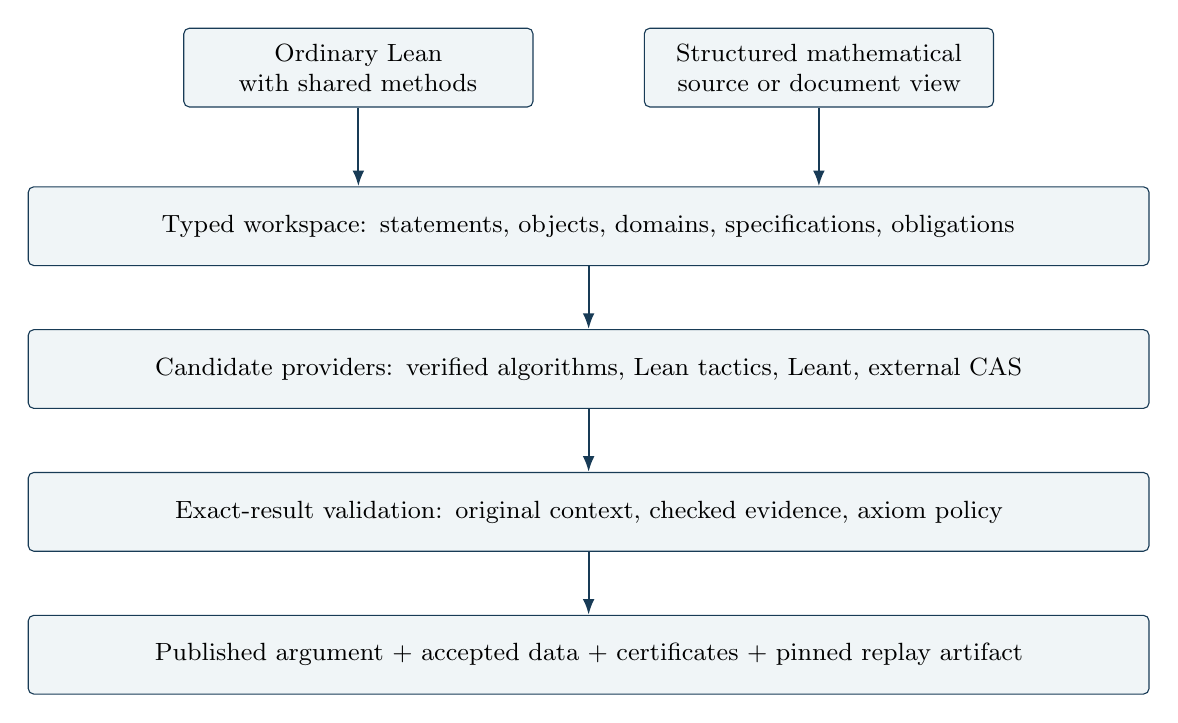
\begin{tikzpicture}[
 box/.style={draw=ink,rounded corners=2pt,fill=pale,align=center,
 minimum height=10mm,text width=42mm,font=\small},
 wide/.style={box,text width=140mm},
 arr/.style={-{Latex[length=2mm]},thick,draw=ink},node distance=8mm]
 \node[box] (lean) {Ordinary Lean\\with shared methods};
 \node[box,right=14mm of lean] (surface) {Structured mathematical\\source or document view};
 \node[wide,below=10mm of $(lean.south)!0.5!(surface.south)$] (ir)
 {Typed workspace: statements, objects, domains, specifications, obligations};
 \node[wide,below=of ir] (providers)
 {Candidate providers: verified algorithms, Lean tactics, Leant, external CAS};
 \node[wide,below=of providers] (gate)
 {Exact-result validation: original context, checked evidence, axiom policy};
 \node[wide,below=of gate] (artifact)
 {Published argument + accepted data + certificates + pinned replay artifact};
 \draw[arr] (lean.south) -- (ir.north -| lean.south);
 \draw[arr] (surface.south) -- (ir.north -| surface.south);
 \draw[arr] (ir) -- (providers);
 \draw[arr] (providers) -- (gate);
 \draw[arr] (gate) -- (artifact);
\end{tikzpicture}
\caption{Proposed architecture. Provider success is not the publication gate;
validation uses the original typed request. The mathematical source frontend is
optional, and shares its computational infrastructure with ordinary Lean.}
\end{figure}

The initial implementation should remain a Lean package. A new global parser,
an independent elaborator for all mathematics, and a new logical kernel are
unnecessary. Structured steps can first be expressed through Lean syntax
extensions and a generated document view. This makes existing source usable
before a separate language becomes a requirement.

The workspace should own immutable elaborated inputs. It should not repeatedly
reparse a pretty-printed telescope for every provider. Compact Lean-owned
identifiers can reference local expressions while an exported request includes
enough explicit binding structure for independent reconstruction. Closed proof
obligations are formed by abstracting their actual ordered contexts, not by
sorting hypotheses alphabetically.

\Needspace{4\baselineskip}
\subsection{The logical acceptance rule is intentionally modest}
A complete document is accepted only when its final proof has the fixed target,
its declared computed objects have their specified properties, and every
assertion that the document presents as proved has evidence. A proof of the final
theorem which ignores a false intermediate assertion does not rescue the
published document. Unused but true assertions may be marked as unused.

Recursive mathematical definitions and induction remain available through
Lean's checked recursion and induction principles. The workspace must not confuse
an admissible recursive definition with an unresolved cycle of proof debts.

The familiar relative soundness argument then follows from checked theorem
application, dependent substitution, and a final check. There is little value
in presenting that argument as a new foundational theorem. The new proof
obligations in Concord concern the concrete computational specifications,
representation bridges, domain preservation, and correctness of the algorithms
or checkers. Those are the theorems whose implementation would make the hybrid
useful.

Logical validity also does not guarantee statement fidelity or explanatory
quality. Lean's validation guidance explicitly distinguishes the validity of a
proof from the meaning of the formal statement~\cite{leanvalidation}. Concord
keeps both a resolved semantic header and a human-readable rendering, but does
not claim that either removes the need for mathematical review.

\Needspace{4\baselineskip}
\subsection{Three retained forms of evidence}
An accepted computation should retain three complementary forms.
The \emph{mathematical record} contains its original inputs, accepted output,
domain, exact relation, branch policy, and method. The \emph{certificate record}
contains the exact data consumed by a checker, the checker identity and version,
and the theorem relating checker acceptance to the specification. The
\emph{host evidence} contains the accepted proof term or sufficient pinned
proof data for its revalidation. Readable Lean source remains a companion form.

Search-free replay means that discovery providers are not consulted. It does
\emph{not} mean computation-free checking: kernel reduction or deterministic
certificate checking may still perform substantial work. A term containing a
reflected checker can require that checker to reduce again. The artifact should
report this cost rather than imply that retaining a term makes all verification
instantaneous.

For strict term replay, the validator accepts no arbitrary tactic source from
the producer; it checks supplied declarations against a controlled environment.
For certificate replay, it runs a pinned, deterministic certificate interpreter
which constructs evidence and then checks that evidence. A saved tactic script
which invokes open search is a third, weaker reproducibility artifact and must
not be mislabeled as search-free replay.

\Needspace{4\baselineskip}
\subsection{A concrete artifact layout}
\par\smallskip\noindent\begin{minipage}{\linewidth}
\begin{lstlisting}
proof-project/
  document.lean           # Authoring source or Lean companion
  document.concord        # Optional structured source
  semantics.json          # Typed identities and interpretation notices
  objects/                # Exact accepted computational data
  certificates/           # Inputs to pinned checkers
  evidence/               # Host proof evidence and declaration identities
  source-map.json         # Claims, computations, and visible explanations
  environment.lock        # Toolchain, imports, definitions, packages
  audit.json              # Axioms, outcomes, conformance, replay mode
\end{lstlisting}
\end{minipage}\par\smallskip
This is a proposed runtime format, not a description of files generated by the
present article. Its exact serialization is an implementation task. A hash
provides identity and tamper detection relative to trusted metadata; it is not
proof. Imported binary modules also require a trust policy: an opaque compiled
file is not an independently checked theorem merely because its filename is
recorded.

When a library is upgraded, the old artifact remains a claim about its old pinned
environment. Migration must first compare the semantic declarations and then
recheck evidence under the new environment. If old terms and newly elaborated
source disagree, neither is automatically authoritative for the intended new
statement. The migration stops for review. Proof changes may be automatic within
policy; plan, object, and statement changes receive distinct visible diffs, as
synthesis A recommends~\cite{synA}.

\Needspace{4\baselineskip}
\subsection{Operational safety and privacy}
An external provider can be mathematically untrusted and still execute dangerous
code. Its process therefore receives only the permissions needed for the request,
and a remote CAS does not receive private definitions or full contexts without
an explicit project policy. Read-only filesystem access, bounded resources, and
no implicit network access are sensible defaults for a local computation worker.

These engineering protections are not new logical axioms. They protect the
user's environment and interactive state. The validator must also obtain the
intended target from a source outside the producer's authority, so that a producer
cannot make a false result appear checked by replacing the target with
\code{True}. The operational boundary and the statement boundary solve different
problems and both belong in a deployed system.

\Needspace{7\baselineskip}
\section{A bounded implementation plan}
\label{sec:plan}
\Needspace{4\baselineskip}
\subsection{First slice: one honest computed object}
The first end-to-end slice should be domain-preserving rational simplification
with complete solving of small univariate examples. It is small enough to
specify fully and rich enough to test the central contribution. It includes a
partial-expression package, a proof-producing polynomial normalizer, exact
input reification, retained domain data, a result contract, and a document view.

The acceptance gate is concrete: the quotient in Section~\ref{sec:domains}
simplifies while retaining its missing point; the complete solution set depends
on the deliberately selected partial or total convention; specialization at the
missing point fails in partial mode. The same operations are available from
ordinary Lean. A broad language with a weak ``verified'' badge is not an
acceptable substitute for this slice.

\Needspace{4\baselineskip}
\subsection{Second slice: a parametric differential certificate}
Implement a small derivative compiler and a polynomial representation package,
then produce the parameterized derivative calculation in
Section~\ref{sec:lambert}. It must handle arbitrary polynomial input and symbolic
$n$, not only output a list of the first few derivatives. The certificate is
connected to ProveIt's actual autonomous theorem under its existing assumptions.

The gate is a replayable proof of the generic step and both branch
instantiations, with no external search during replay. The negative neighbors
alter the recurrence, remove the non-pole hypothesis, and weaken neighborhood
equality to pointwise equality. This gives analysis an early, concrete role,
consistent with the syntheses' concern that analysis plumbing was underrepresented
in some samples~\cite{synA,synB}.

\Needspace{4\baselineskip}
\subsection{Third slice: structural synthesis and independent suggestions}
Connect Leant through the common typed protocol after measuring it on the
structural obligations produced by these two slices. Compare it with direct
lemma application and existing Lean search supplied the same provider inventory.
Repair the displayed-edit replay boundary before advertising independently
verified suggestions.

The gate is interchangeability: disabling Leant must not invalidate a stored
proof; replacing it with another candidate producer must not change acceptance.
A provider timeout, malformed result, or incorrect output should fail locally
without corrupting the current accepted mathematical objects.

\Needspace{4\baselineskip}
\subsection{Fourth slice: representations and finite algebra}
Add the three-view stress test and the binomial-transform example. Verify that
integer coefficient computation acts on arbitrary additive commutative groups
without importing a field requirement. Then add formal jets, with order
propagation and coefficient projection contracts.

The gate is not a fixed promised compression percentage. It is evidence that
these packages remove recurring author work, expose better failure messages,
and preserve theorem generality under controlled edits. Helpers and package
maintenance are charged equally to the ordinary-Lean comparison.

\Needspace{4\baselineskip}
\subsection{What should be deliberately deferred}
A general natural-language definition parser, universal simplification of
transcendental expressions, arbitrary certified symbolic integration, global
conditional equality saturation, cross-foundation proof transport, and automatic
observational replacement of arbitrary witnesses should not be initial
requirements. None is needed to test the proposed central interface.

The most dangerous implementation trap is to build many attractive verbs whose
actual contract is ``try a large tactic and print success.'' A smaller family of
operations with exact data, domain, and result guarantees would be a more useful
second-round outcome.

\Needspace{7\baselineskip}
\section{Evaluation: isolate the language from the mathematics}
\label{sec:evaluation}
\Needspace{4\baselineskip}
\subsection{Comparison conditions}
An evaluation should separate original code, improved mathematical libraries,
improved algorithms, and the new authoring surface. At minimum, compare:
\begin{center}
\begin{tabularx}{\textwidth}{@{}L{.09\textwidth}Y@{}}
\toprule
Arm & Configuration \\
\midrule
A & Original ProveIt Lean as a historical reference, not the sole baseline.\\
B & Refactored Lean with the same theorem wrappers, verified algorithms,
certificate checkers, and allowed search inventory as Concord.\\
C & Arm B with a generated mathematical document view and retained computation
records, but ordinary Lean authoring.\\
D & The proposed mathematical source frontend over exactly the same backend as
B and C.\\
\bottomrule
\end{tabularx}
\end{center}
The difference between A and B estimates the combined library and automation
improvement, not a language advantage. The difference between B and C tests the
value of presentation and accounting. The difference between C and D tests
whether the new input form is worth learning. A second ablation should enable
or disable the new CAS method while holding the frontend fixed.

The target theorem, aliases that expose it, and its downstream closure must be
excluded from discovery. A search service that simply retrieves the theorem
being reconstructed invalidates the comparison. Cached target-specific results
must be handled by the same exclusion policy. Split by theorem families or
modules, rather than random neighboring proof lines, to reduce leakage through
near-identical lemmas.

\Needspace{4\baselineskip}
\subsection{Measure authoring, reading, computation, and maintenance separately}
Authoring measures should include time to a checked result, number of explicit
mathematical choices, number of attempts, manual refinement of guards, and time
spent diagnosing failure. Reader tasks should ask participants to identify the
main invariant, explain why a domain condition is necessary, and predict the
failure caused by a nearby mutation. Agreement with a stylistic preference survey
alone would be weak evidence.

Computation measures include elaboration time, search time, certificate generation,
certificate size, and replay time, with failures and high-percentile costs
reported. Maintenance measures include changes needed after a theorem wrapper,
instance, representation route, or library revision changes. The cost of writing
and maintaining a domain package must be amortized over its actual uses, not
hidden outside the accounting.

A useful error measure is \emph{contract surprise}: the fraction of operations
whose displayed guarantees a reader overestimates. Asking whether a returned
factorization is irreducible, whether a jet is an infinite solution, and whether
a missing branch is covered directly tests the intended value of the interface.
Another is \emph{guard surprise}: whether the author can predict which
specializations remain legal after a calculation.

\Needspace{4\baselineskip}
\subsection{Negative neighbors are executable specifications}
The following are proposed acceptance tests for an implementation, not claims
that a Concord implementation already passed them. The companion Python script
checks selected arithmetic examples only.
\begin{longtable}{@{}L{.07\textwidth}L{.47\textwidth}L{.38\textwidth}@{}}
\toprule
ID & Mutation or failure & Required behavior \\
\midrule
\endhead
D1 & Cancel $(x^2-1)/(x-1)$ and evaluate the partial result at $1$ & Retain the
excluded point; reject the evaluation.\\
D2 & Use a partial-function solution certificate for the totalized equation &
Reject the semantic mismatch; the complete solution sets differ.\\
D3 & Solve $ax=0$ as $\{0\}$ without considering $a=0$ & Report a conditional
answer or require branch coverage.\\
D4 & Substitute a value at which an inherited guard fails & Reinstantiate the
guard and locate its origin; do not use the cached equality unconditionally.\\
C1 & Verify only that returned factors multiply to the input & Do not label them
irreducible without further evidence.\\
C2 & Verify every proposed root, but omit one & Accept only root soundness;
reject a complete-answer claim.\\
C3 & Supply a tiny floating residual for an exact identity & Treat it as a
candidate diagnostic, not proof.\\
C4 & Use a Gr\"obner membership witness with rational coefficients over $\Z$ &
Reject the coefficient-domain mismatch.\\
V1 & Cast $a\dot-b$ to $a-b$ without $b\le a$ & Keep the guard or select an
explicit alternative representation.\\
V2 & Add a competing representation route & Preserve the old route or request
a visible selection; never choose by provability.\\
V3 & Cancel a nonzero nonunit in a ring with zero divisors & Require the actual
cancellation capability.\\
A1 & Change $3n+2$ to $3n+1$ in the Lambert recurrence & Reject the symbolic
numerator identity.\\
A2 & Remove $W(x)\ne-1$ from the analytic instantiation & Expose the unresolved
requirement without strengthening the target.\\
A3 & Differentiate from equality at one point only & Require neighborhood
equality or a different valid theorem.\\
F1 & Omit the upper endpoint in a finite reindexing & Fail coverage.\\
F2 & Treat a finite jet certificate as a full formal identity & Reject the
relation-strength mismatch.\\
L1 & Provider returns a different expression with the same printed name &
Reject incorrect typed origin binding.\\
L2 & Displayed replacement differs from the probed tactic & Independently replay
the exact replacement before giving it a replay receipt.\\
L3 & A request times out or a status field is missing & Return exhaustion or a
protocol error, never completion or refutation.\\
L4 & Two children commit incompatible shared data & Reject the combined transaction.\\
P1 & A false intermediate claim is unused by the final proof & Reject document
completion despite the final theorem's proof.\\
P2 & A transitive dependency uses an unapproved axiom & Fail the declared publication
policy.\\
P3 & A library update changes the resolved statement but preserves its spelling &
Invalidate migration and display a semantic change.\\
\bottomrule
\end{longtable}

\Needspace{4\baselineskip}
\subsection{Stopping rules}
If the computational packages are useful but the new syntax does not improve
authoring or comprehension, ship the packages and the document view. If explicit
guards create more confusion than they prevent, improve their grouping and
rendering rather than deleting their semantics. If a verified algorithm is too
expensive for interactive use, retain it as a reference and investigate a
certificate-producing external implementation with the same contract.

Success is not the existence of a language bearing a new name. It is a measured
reduction in the cost of developing, checking, understanding, and maintaining
the intended mathematics, without relocating that cost into unreported
infrastructure or unexamined assumptions.

\Needspace{7\baselineskip}
\section{Decisions for the second brainstorm iteration}
\label{sec:decisions}
The following answers consolidate the concrete questions in both syntheses.
They are design choices to test, rather than claims that the associated engineering
has already been completed~\cite{synA,synB}.

\begin{longtable}{@{}L{.30\textwidth}L{.62\textwidth}@{}}
\toprule
Open question & Proposed decision and discriminating evidence \\
\midrule
\endhead
Is the language an input form or a document? & Both frontends share the same
workspace. Compare a generated view with authored structured source before
making the latter mandatory.\\
What is the smallest useful method? & A project-owned theorem interface with
role annotations for logical steps; a result contract plus a verified algorithm
or checker for computation. Demonstrate one end-to-end rational example first.\\
Must the displayed reason constrain the proof? & Yes when it states a particular
method. Keep an explicitly unconstrained search form. Test that a correct but
different proof triggers a reason change.\\
Which choices may be automatic? & Proof evidence within a fixed contract may be
replaced under policy. New accepted data, branches, plans, and statements are
visible changes.\\
How are view chains composed? & Retain the actual intermediate objects and
instantiate every guard along the route. Begin with equality-based denotations;
require explicit routes or checked coherence.\\
Where does definition authoring start? & With partial-expression and polynomial
representation packages. Compare downstream work against alternate ordinary
Lean representations under the same specification.\\
How are changing theorem binders handled? & Register roles on maintained semantic
wrappers. Recheck wrapper types and test migration; do not infer meaning from
binder position.\\
How are semantic notices dismissed? & Record a dismissal against the resolved
construction and selected convention. Invalidate it when that meaning changes;
measure false alarms. A dismissed notice never discharges a method obligation.\\
What does verified suggestion mean? & Distinguish probe acceptance, exact-edit
replay, result certification, and document completion. Test malformed and
partial responses.\\
What is the provider's negative interface? & Return search status and abstraction
loss metadata, but require actual evidence and a proved bridge for mathematical
nonexistence.\\
Is Leant worth an adapter? & Measure its contribution on multi-step structural
assembly against equally equipped Lean search. Do not assume every
\code{exact} line is a synthesis opportunity.\\
What is the unit of replay? & A typed mathematical node plus its accepted data and
evidence under a pinned environment. Terms and portable certificates have
explicitly different replay modes.\\
Must discarded data candidates be published? & No. Publish the accepted value and
its specification; retain optional exploration logs separately under privacy
policy.\\
Who owns competing method packages? & Semantic interfaces have owners and explicit
versions. Conflicting interpretations need qualification, not import-order
precedence.\\
How is infrastructure cost charged? & Share every wrapper, algorithm, and checker
with the Lean baseline; report construction and maintenance effort.\\
What would justify abandoning the surface? & Evidence that the packages and view
help but a new input form does not. A library-and-tooling outcome is an explicit
success condition.\\
\bottomrule
\end{longtable}

\Needspace{7\baselineskip}
\section{The remaining research questions}
\label{sec:research}
The most promising research problem is \emph{demand-directed certification}.
A consumer should state what it needs from a computed object, and the system
should seek no stronger certificate than necessary. If a proof only needs a
polynomial consequence, a membership identity may be enough; proving a full
Gr\"obner basis is wasted effort. If a proof later needs completeness, the same
accepted object can acquire an additional property without changing its identity.
This requires a library of proved implications between result contracts, not a
heuristic confidence hierarchy.

A second problem is \emph{computation-aware explanation}. A factorization trace
may be enormous, but the useful mathematical reason may be ``this product gives
the two real roots, and the other factors have no real zeros.'' An explanation
should summarize the certified properties actually used. Method conformance can
check that a displayed construction follows a specified interface, but it cannot
by itself prove that the explanation is pedagogically good. Reader tasks must
supply that evidence.

A third problem is \emph{domain minimization with proofs}. A computation can start
with conservative guards and later prove that some are unnecessary, or replace a
conditional expression with a piecewise one covering more of the domain. These
operations should have their own certificates. They are attractive because they
improve mathematical usability without sacrificing exactness, but no general
algorithm for weakest domain conditions is assumed.

A fourth problem is \emph{representation choice under a stable specification}.
Sparse and dense polynomial forms, algebraic-number encodings, and alternative
formal-series representations can have very different computational costs.
A verified refinement interface can permit implementation changes while
preserving the public object. Optimizing this choice without hiding changes to
accepted data or observations is a substantive compiler problem.

Finally, \emph{proof extraction from existing developments} can make adoption
incremental. Existing \code{have} chains, calculations, and recognizable
computational fragments can be lifted into workspace nodes. The extracted view
should initially preserve the exact proof rather than invent an alleged author
intention. User edits can then group or name meaningful steps. This would also
provide a realistic corpus for evaluating whether the proposed units match
mathematicians' actual working patterns.

\Needspace{7\baselineskip}
\section{Conclusion}
The first iteration found a sound foundation for a readable Lean-facing proof
layer. The most useful second step is not another set of near-synonymous proof
verbs. It is to make \emph{certified mathematical computation} a first-class part
of that layer.

Concord would let the author select an object, a domain, a representation, or an
ansatz, then ask for computational consequences with explicit guarantees. A
verified algorithm can produce a result; an external CAS can suggest one; Leant
can assemble the logical connections. None receives authority to alter the
intended statement or inflate the strength of a returned certificate.

The Lambert example shows the intended division of labor. A reusable symbolic
calculation establishes the polynomial differential recurrence. A local analytic
theorem transports that calculation through a solution of an autonomous equation.
Branch hypotheses remain visible, and the same computation serves both branches.
The rational-expression example shows why the interface must also preserve
meaning: dropping a domain can change a complete solution set even when a
familiar cancellation is valid wherever it was originally defined.

The proposed system is ambitious in its mathematical interface but conservative
in its foundations and initial scope. Its first deliverables should be small
verified computational packages, exact result contracts, and readable retained
evidence. A new authoring language is justified only to the extent that it makes
those capabilities easier to use and the resulting mathematics easier to
understand.

\appendix
\Needspace{7\baselineskip}
\section{Minimal protocol and semantic interfaces}
\label{app:interfaces}
The following Lean-like type sketches describe interfaces; they are not compiled
source in this deliverable. Universe parameters, serialization, and operational
metadata would be supplied by an implementation.
\par\smallskip\noindent\begin{minipage}{\linewidth}
\begin{lstlisting}
structure Certified (A : Type u) (P : A -> Prop) where
  value : A
  evidence : P value

structure ConditionalResult (A : Type u) (P : A -> Prop) where
  guard : Prop
  value : A
  evidence : guard -> P value

structure CheckedAlgorithm (I : Type u) (O : I -> Type v)
    (spec : (x : I) -> O x -> Prop) where
  run : (x : I) -> O x
  correct : (x : I) -> spec x (run x)

structure CertificateInterface (I : Type u) (O : I -> Type v)
    (C : (x : I) -> O x -> Type w)
    (spec : (x : I) -> O x -> Prop) where
  check : (x : I) -> (y : O x) -> C x y -> Bool
  sound : (x : I) -> (y : O x) -> (c : C x y) ->
    check x y c = true -> spec x y
\end{lstlisting}
\end{minipage}\par\smallskip
The constant-value conditional interface is adequate when the returned symbolic
representation exists independently of its guard. For an object whose type or
construction itself depends on a guard witness, use a dependent function or
scoped branch instead; the displayed simplified interface must not erase that
dependency.

A provider does not create a trusted \code{Certified} value by emitting JSON
with an \code{evidence} field. The host parses the returned data, checks the
relation to the original input, reconstructs the alleged evidence, and checks
its type and dependencies. Callback receipts and logical evidence are distinct
objects.

A minimal proposed surface grammar is:
\par\smallskip\noindent\begin{minipage}{\linewidth}
\begin{lstlisting}
document    ::= declaration*
declaration ::= context | definition | theorem | computation
context     ::= "context" name ":" scoped_declaration*
computation ::= "calculate" name ":=" request contract_clause*
step        ::= claim | obtain | computation | cases | induction
              | calculation_chain | lean_escape
claim       ::= "have" name ":" proposition justification
contract_clause ::= "on" domain | "preserving domain"
                  | "completely" | "modulo" precision
                  | "satisfying" specification
justification ::= "by" method input_clause* | "by search" policy
\end{lstlisting}
\end{minipage}\par\smallskip
Formulas initially reuse Lean's term elaboration. The grammar is intentionally
small; the result contracts and the typed method registry determine what each
operation means. New notation is a package feature, not a source of permission
for search to reinterpret a formula.

\Needspace{7\baselineskip}
\section{Source register and inspection boundaries}
\label{app:sources}
\Needspace{4\baselineskip}
\subsection{Pinned repository revisions}
\Needspace{4\baselineskip}\textbf{Brainstorm.}\par
\code{494be9d5ab41a5ae219fc6f800e6aee3c93bce39}.
Both requested synthesis sources were read, including their comparative
assessments, Leant discussion, proposed experiments, and next-iteration questions.
Individual proposals were used through those reports' detailed accounts; this
article does not claim an independent full rereading of all nine originals.
\par\Needspace{4\baselineskip}\textbf{ProveIt.}\par
\code{24ce8bd743eaab64a91ce90725ea00f498d319d2}.
Direct static inspection covered the three modules listed below. Synthesis B's
corpus audit used local revision \code{7c4e3f10}; its statistics are attributed
rather than asserted as a new measurement at this review's public ref.
\par\Needspace{4\baselineskip}\textbf{Leant.}\par
\code{3a40904be8a410d832d9ab6900b3d3e7b425eccb}.
Direct static inspection covered the verification receipt boundary, the engine's
interface and module commentary, and relevant tactic-suggestion and applied-edit
code in \code{Main.hs}. Uncommitted behavioral work discussed in the syntheses
was not executed or verified here.


\Needspace{4\baselineskip}
\subsection{Inspected file locators}
The ProveIt module root is
\path{Analysis/FabiusFunction/Lean/FabiusFunction/}. Under it, the reviewed files
are \path{AutonomousIteratedDeriv.lean}, \path{BinomialInversion.lean}, and
\path{LambertWHigherDerivatives.lean}. The article's analysis uses their actual
mathematical decomposition, not an assumption that every long proof can be
compressed automatically.

The Leant paths are \path{src/Leant/Synth/Verification.hs},
\path{src/Leant/Synth/Engine.hs}, and \path{src/Main.hs}. In the last file, the
review focused on source lines 4600--4760 and 4820--5110 at the pinned revision:
response parsing, displayed suggestions, bounded probes, chaining, and storing
applied edits. No claim is made that the Haskell project was built or that the
live backend was exercised.

The bibliography links every repository item to its pinned revision. External
manuals and current documentation were consulted on September 5, 2026, Pacific
time. The moving Lean reference identified itself as covering version
\code{4.34.0-rc2}; that is documentation context, not a claimed ProveIt toolchain
or a tested compatibility target~\cite{leanintro}.

\Needspace{7\baselineskip}
\section{Companion calculations and limits of validation}
\label{app:checks}
The archive includes \path{check_examples.py} and its recorded output
\path{example_checks.json}. The script uses Python integers and exact rational
arithmetic from the standard library. It checks polynomial product identities,
the first Lambert recurrence values, a coefficient identity in a symbolic
parameter, finite derivative-numerator instances, the formal-series jet residual,
integer square-root bounds, and several nearby false variants.

The execution recorded \textbf{27 of 27 checks passed}. That result is a test of
the supplied arithmetic examples and the script, not a formal proof of the
script's correctness. It is not an evaluation of Concord, a Leant integration,
or a Lean kernel certificate. The universal arguments about partial-expression
composition, the derivative family, and the formal-series solution are proved
mathematically in the article; they have not been compiled as new Lean theorems
in this deliverable.

The article therefore makes three different claims with different support:
observations about repository code are based on pinned static reads; the language
and protocol are proposed designs; and the arithmetic supplement was actually
executed. Keeping these claims separate is itself an instance of the result
contract discipline advocated throughout the article.

\Needspace{8\baselineskip}
\phantomsection
\addcontentsline{toc}{section}{References}
\begin{thebibliography}{99}
\small
\bibitem{synA}
Codex. \emph{Mathematical Ideas, Checked Evidence: A Unified Evaluation of Nine
Proof-Language Proposals}. Brainstorm synthesis, September 5, 2026.
\url{https://github.com/VladimirReshetnikov/Brainstorm/blob/494be9d5ab41a5ae219fc6f800e6aee3c93bce39/docs/synthesis/unified-report.tex}.

\bibitem{synB}
Claude (Anthropic). \emph{Nine Blueprints for a Mathematician's Proof Language
over Lean}. Brainstorm synthesis, revised September 5, 2026.
\url{https://github.com/VladimirReshetnikov/Brainstorm/blob/494be9d5ab41a5ae219fc6f800e6aee3c93bce39/docs/unified_report/unified_report.tex}.

\bibitem{pautonomous}
Vladimir Reshetnikov and contributors. \emph{ProveIt:
AutonomousIteratedDeriv.lean}. Source inspected at revision \code{24ce8bd7}.
\url{https://github.com/VladimirReshetnikov/ProveIt/blob/24ce8bd743eaab64a91ce90725ea00f498d319d2/Analysis/FabiusFunction/Lean/FabiusFunction/AutonomousIteratedDeriv.lean}.

\bibitem{pbinomial}
Vladimir Reshetnikov and contributors. \emph{ProveIt: BinomialInversion.lean}.
Source inspected at revision \code{24ce8bd7}.
\url{https://github.com/VladimirReshetnikov/ProveIt/blob/24ce8bd743eaab64a91ce90725ea00f498d319d2/Analysis/FabiusFunction/Lean/FabiusFunction/BinomialInversion.lean}.

\bibitem{plambert}
Vladimir Reshetnikov and contributors. \emph{ProveIt:
LambertWHigherDerivatives.lean}. Source inspected at revision \code{24ce8bd7}.
\url{https://github.com/VladimirReshetnikov/ProveIt/blob/24ce8bd743eaab64a91ce90725ea00f498d319d2/Analysis/FabiusFunction/Lean/FabiusFunction/LambertWHigherDerivatives.lean}.

\bibitem{lverify}
Vladimir Reshetnikov and contributors. \emph{Leant: Verification.hs}.
Source inspected at revision \code{3a40904b}.
\url{https://github.com/VladimirReshetnikov/Leant/blob/3a40904be8a410d832d9ab6900b3d3e7b425eccb/src/Leant/Synth/Verification.hs}.

\bibitem{lengine}
Vladimir Reshetnikov and contributors. \emph{Leant: Engine.hs}.
Source inspected at revision \code{3a40904b}.
\url{https://github.com/VladimirReshetnikov/Leant/blob/3a40904be8a410d832d9ab6900b3d3e7b425eccb/src/Leant/Synth/Engine.hs}.

\bibitem{lmain}
Vladimir Reshetnikov and contributors. \emph{Leant: Main.hs}.
Source inspected at revision \code{3a40904b}, especially the suggestion and
applied-tactic paths.
\url{https://github.com/VladimirReshetnikov/Leant/blob/3a40904be8a410d832d9ab6900b3d3e7b425eccb/src/Main.hs}.

\bibitem{leanvalidation}
The Lean development team. \emph{Validating a Lean Proof}. Lean Language Reference.
\url{https://lean-lang.org/doc/reference/latest/ValidatingProofs/}.
Accessed September 5, 2026.

\bibitem{leanaxioms}
The Lean development team. \emph{Axioms}, especially ``Creating and Tracking
Proofs That Trust the Compiler'' and ``Axioms and the native\_decide Tactic.''
Lean Language Reference.
\url{https://lean-lang.org/doc/reference/latest/Axioms/}.
Accessed September 5, 2026.

\bibitem{leancbv}
The Lean development team. \emph{Tactic Reference} and \emph{Lean 4.30.0 release
notes}, concerning call-by-value proof-layer simplification.
\url{https://lean-lang.org/doc/reference/latest/Tactic-Proofs/Tactic-Reference/};
\url{https://lean-lang.org/doc/reference/latest/releases/v4.30.0/}.
Accessed September 5, 2026.

\bibitem{leanintro}
The Lean development team. \emph{Introduction}. Lean Language Reference,
version identified by the consulted page as \code{4.34.0-rc2}.
\url{https://lean-lang.org/doc/reference/latest/Introduction/}.
Accessed September 5, 2026.

\bibitem{module}
Mathlib contributors. \emph{Mathlib.Tactic.Module}: \code{match_scalars} and
\code{module}.
\url{https://leanprover-community.github.io/mathlib4_docs/Mathlib/Tactic/Module.html}.
Accessed September 5, 2026.

\bibitem{polyrith}
Mathlib contributors. \emph{Mathlib.Tactic.Polyrith}. Current documentation notes
that the external service is no longer available and the tactic is unsupported.
\url{https://leanprover-community.github.io/mathlib4_docs/Mathlib/Tactic/Polyrith.html}.
Accessed September 5, 2026.

\bibitem{davenport}
James H. Davenport. \emph{Towards Verified Polynomial Factorisation}.
arXiv:2409.09533v1, September 14, 2024.
\url{https://arxiv.org/abs/2409.09533}.

\bibitem{shen}
Hao Shen, Junyu Guo, Junqi Liu, and Lihong Zhi.
\emph{Automated Tactics for Polynomial Reasoning in Lean 4}.
arXiv:2604.13514v1, April 15, 2026.
\url{https://arxiv.org/html/2604.13514v1}.

\bibitem{berlekamp}
Jose Divas\'on, Sebastiaan J. C. Joosten, Ren\'e Thiemann, and Akihisa Yamada.
\emph{The Factorization Algorithm of Berlekamp and Zassenhaus}.
Archive of Formal Proofs, October 14, 2016, with subsequent revisions.
\url{https://isa-afp.org/entries/Berlekamp_Zassenhaus.html}.
See also \emph{A Verified Implementation of the Berlekamp--Zassenhaus
Factorization Algorithm}, Journal of Automated Reasoning 64, 699--735,
\url{https://doi.org/10.1007/s10817-019-09526-y}.

\bibitem{interval}
Guillaume Melquiond and contributors. \emph{Interval Package for Rocq}.
Official documentation, accessed September 5, 2026.
\url{https://coqinterval.gitlabpages.inria.fr/}.

\bibitem{isar}
Makarius Wenzel and Isabelle contributors. \emph{Isar: Intelligible
semi-automated reasoning}. Official project description.
\url{https://isabelle.in.tum.de/Isar/}.
Accessed September 5, 2026.
\end{thebibliography}
\end{document}
